\documentclass{classrep}
\usepackage[utf8]{inputenc}
\frenchspacing

\usepackage{graphicx}
\usepackage[usenames,dvipsnames]{color}
\usepackage[hidelinks]{hyperref}
\usepackage{lmodern}
\usepackage{graphicx}
\usepackage{placeins}
\usepackage{url}
\usepackage{amsmath, amssymb, mathtools}
\usepackage{listings}
\usepackage{fancyhdr, lastpage}
\usepackage{rotating}
\usepackage{makecell}

\pagestyle{fancyplain}
\fancyhf{}
\renewcommand{\headrulewidth}{0pt}
\cfoot{\thepage\ / \pageref*{LastPage}}

%--------------------------------------------------------------------------------------%
\studycycle{Informatyka stosowana, studia dzienne, II st.}
\coursesemester{I}

\coursename{Wprowadzenie do Data Science i metod uczenia maszynowego}
\courseyear{2020/2021}

\courseteacher{mgr inż. Rafał Woźniak}
\coursegroup{Wtorek, 13:15}

\author{%
    \studentinfo[239661@edu.p.lodz.pl]{Szymon Gruda}{239661}\\
    \studentinfo[239671@edu.p.lodz.pl]{Jan Karwowski}{239671}\\
    \studentinfo[239673@edu.p.lodz.pl]{Michał Kidawa}{239673}\\
    \studentinfo[216806@edu.p.lodz.pl]{Kamil Kowalewski}{239676}\\
}

\title{Zadanie 2.: Problem Set 2}

\begin{document}
    \maketitle
    \thispagestyle{fancyplain}

    \newpage
    \tableofcontents
    \newpage

    \section{Wprowadzenie}
    \label{intro} {
        Jednym z elementów przygotowania danych do późniejszej analizy jest rozwiązanie
        problemu brakujących, a niezbędnych do analizy atrybutów. Jest to realizowane
        poprzez imputację danych. W tym zadaniu badany był wpływ imputacji,
        przeprowadzonej przy pomocy różnych metod, na statystyki dotyczące zbioru
        danych. Jako testowy zbiór danych wykorzystaliśmy zbiór
        \textit{heart-disease-uci} \cite{dataset}. Tabela \ref{opis-zbioru-danych}
        zawiera opis zawartości tego zbioru.
        
        \begin{sidewaystable}[!htbp]
            \centering
            \begin{tabular}{|c|c|}
                \hline
                Nazwa kolumny & Opis zawartości \\ \hline
                age & wiek w latach   \\ \hline
                sex & płeć, gdzie 1 to mężczyzna a 0 to kobieta  \\ \hline
                cp (chest-pain-type) & rodzaj bólu w klatce piersiowej, przyjmuje wartość 0, 1, 2 lub 3  \\ \hline
                trestbps (resting-blood-pressure) & ciśnienie krwi w czasie spoczynku (w mm/Hg przy przyjęciu do szpitala) \\ \hline
                chol (serum-cholestoral) & cholesterol w surowicy w mg/dl  \\ \hline
                fbs (fasting-blood-sugar) & \makecell{poziom cukru we krwi na czco, przyjmuje wartość 1 dla \\ poziomu większego niż 120 mg/dl, lub wartość 0 dla poziomu mniejszego}  \\ \hline
                restecg (resting-electrocardiographic) & wyniki eloktrokardiografu w stanie spoczynku, przyjmuje wartość 0, 1 lub 2   \\ \hline
                thalach (maximum-heart-rate) & najwyższe osiągnięte tętno   \\ \hline
                exang (exercise-induced-angina) & \makecell{dławica wysiłkowa, przyjmuje wartość 1, jeżeli dławica występuje, \\ w przeciwnym razie przyjmuje wartość 0}   \\ \hline
                oldpeak & Obniżenie odcinka ST, wywołane przez ćwiczenie, w stosunku do odpoczynku   \\ \hline
                slope (the-slope-of-the-peak-exercise) & nachylenie szczytowe odcinka ST podczas wysiłku, przyjmuje wartość 0, 1 lub 2  \\ \hline
                ca (number-of-major-vessels) & liczba głównych naczyń, przyjmuje wartość 0, 1, 2, 3 lub 4  \\ \hline
                thal & przyjmuje wartość 0, 1, 2 lub 3   \\ \hline
                target & przyjmuje wartość 0 lub 1 \\ \hline
            \end{tabular}
            \caption{Opis zbioru danych}
            \label{opis-zbioru-danych}
        \end{sidewaystable}
        \FloatBarrier
        Imputację stosujemy dla kilku wariantów zbioru, w których braki danych zostały
        usunięte poprzez losowe usunięcie kolejno 5\%, 15\%, 30\% i 45\% danych. Dla
        analizy wpływu imputacji zostały obliczone statystyki takie jak: średnia
        arytmetyczna, odchylenie standardowe, moda, mediana oraz kwartyle. Ich wartości
        zostały wyznaczone dla zbioru, zawierającego wszystkie dane, a także dla
        zbiorów, których brakujące dane zostały uzyskane wypełnione danymi uzyskanymi
        przy użyciu następujących metod imputacji: "mean imputation", interpolacji,
        hot-deck, krzywej regresji.
        
        Po zapoznaniu się z charakterystyką zbioru danych postawiliśmy trzy hipotezy:
        \begin{itemize}
            \item średnia wieku osoby chorej na serce jest równa 54 (lata)
            \item średnie ciśnienie spoczynkowe osoby chorej wynosi 131
            \item średnie maksymalne zanotowane tętno wynosi 148
        \end{itemize}
    }

    \section{Wyniki}
    \label{results} {

        \subsection{Braki w danych 5\%}
        \label{results:5-percent} {

            \subsubsection{List wise deletion}
            \label{results:5-percent:list-wise} {

                \begin{table}[!htbp]
                    \centering
                    \begin{tabular}{|c|c|c|c|c|c|c|}
                        \hline
                        & Mean & Std & Mode & Q1 & Median & Q3 \\ \hline
                        age & 54.2838 & 9.2744 & 58.0 & 47.75 & 56.0 & 60.0 \\ \hline
                        sex & 0.6824 & 0.4671 & 1.0 & 0.0 & 1.0 & 1.0 \\ \hline
                        chest-pain-type & 0.8514 & 0.9715 & 0.0 & 0.0 & 0.0 & 2.0 \\ \hline
                        resting-blood-pressure & 131.0068 & 16.7858 & 120.0 & 120.0 & 130.0 & 140.0 \\ \hline
                        serum-cholestoral & 249.6351 & 55.9982 & 197.0 & 210.75 & 243.5 & 275.0 \\ \hline
                        fasting-blood-sugar & 0.1554 & 0.3635 & 0.0 & 0.0 & 0.0 & 0.0 \\ \hline
                        resting-electrocardiographic & 0.5068 & 0.5408 & 0.0 & 0.0 & 0.0 & 1.0 \\ \hline
                        maximum-heart-rate & 148.0676 & 23.2554 & 143.0 & 131.0 & 151.5 & 166.0 \\ \hline
                        exercise-induced-angina & 0.3243 & 0.4697 & 0.0 & 0.0 & 0.0 & 1.0 \\ \hline
                        oldpeak & 1.0108 & 1.0793 & 0.0 & 0.0 & 0.65 & 1.6 \\ \hline
                        the-slope-of-the-peak-exercise & 1.3716 & 0.598 & 1.0 & 1.0 & 1.0 & 2.0 \\ \hline
                        number-of-major-vessels & 0.7568 & 1.0408 & 0.0 & 0.0 & 0.0 & 1.0 \\ \hline
                        thal & 2.3108 & 0.5931 & 2.0 & 2.0 & 2.0 & 3.0 \\ \hline
                        target & 0.5135 & 0.5015 & 1.0 & 0.0 & 1.0 & 1.0 \\ \hline
                    \end{tabular}
                    \caption{}
                    \label{result_5_List-wise-deletion}
                \end{table}
                \FloatBarrier

                \begin{figure}[!htbp]
                    \centering
                    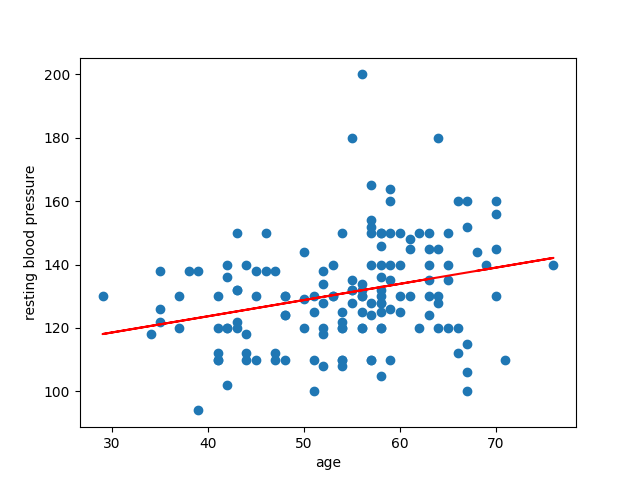
\includegraphics
                    [width=\textwidth,keepaspectratio]
                    {img/regression-5-List-wise-deletion-resting-blood-pressure-age.png}
                    \caption
                    [regression-5-List-wise-deletion-resting-blood-pressure-age]
                    {Współczynnik kierunkowy: 0.5113, Punkt przecięcia: 103.2523}
                    \label{regression-5-List-wise-deletion-resting-blood-pressure-age}
                \end{figure}
                \FloatBarrier


                \begin{figure}[!htbp]
                    \centering
                    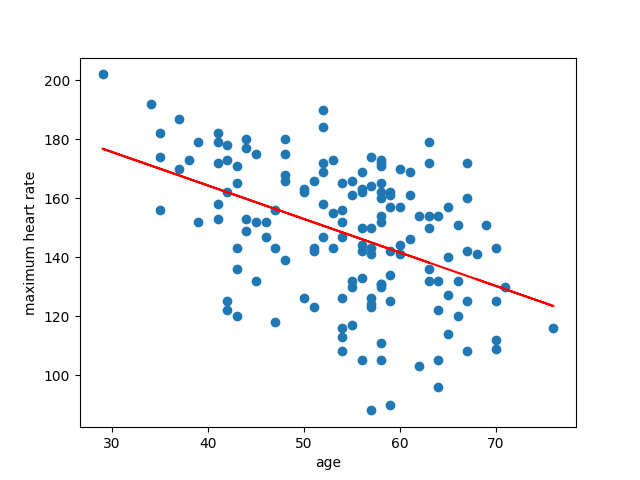
\includegraphics
                    [width=\textwidth,keepaspectratio]
                    {img/regression-5-List-wise-deletion-maximum-heart-rate-age.png}
                    \caption
                    [regression-5-List-wise-deletion-maximum-heart-rate-age]
                    {Współczynnik kierunkowy: -1.1359, Punkt przecięcia: 209.7261}
                    \label{regression-5-List-wise-deletion-maximum-heart-rate-age}
                \end{figure}
                \FloatBarrier

            }

            \subsubsection{Mean imputation}
            \label{results:5-percent:mean-input} {

                \begin{table}[!htbp]
                    \centering
                    \begin{tabular}{|c|c|c|c|c|c|c|}
                        \hline
                        & Mean & Std & Mode & Q1 & Median & Q3 \\ \hline
                        age & 54.3024 & 8.7404 & 58.0 & 48.0 & 55.0 & 60.0 \\ \hline
                        sex & 0.6964 & 0.4606 & 1.0 & 0.0 & 1.0 & 1.0 \\ \hline
                        chest-pain-type & 0.9934 & 1.0 & 0.0 & 0.0 & 1.0 & 2.0 \\ \hline
                        resting-blood-pressure & 131.3514 & 17.0986 & 120.0 & 120.0 & 130.0 & 140.0 \\ \hline
                        serum-cholestoral & 245.9397 & 51.0872 & 245.9397 & 211.5 & 244.0 & 272.0 \\ \hline
                        fasting-blood-sugar & 0.132 & 0.3391 & 0.0 & 0.0 & 0.0 & 0.0 \\ \hline
                        resting-electrocardiographic & 0.5578 & 0.5234 & 1.0 & 0.0 & 1.0 & 1.0 \\ \hline
                        maximum-heart-rate & 149.4913 & 22.4148 & 149.4913 & 136.5 & 151.0 & 165.0 \\ \hline
                        exercise-induced-angina & 0.3036 & 0.4606 & 0.0 & 0.0 & 0.0 & 1.0 \\ \hline
                        oldpeak & 1.0287 & 1.1035 & 0.0 & 0.0 & 0.8 & 1.6 \\ \hline
                        the-slope-of-the-peak-exercise & 1.3927 & 0.6042 & 1.0 & 1.0 & 1.0 & 2.0 \\ \hline
                        number-of-major-vessels & 0.7195 & 0.9476 & 0.0 & 0.0 & 0.0 & 1.0 \\ \hline
                        thal & 2.2871 & 0.5869 & 2.0 & 2.0 & 2.0 & 3.0 \\ \hline
                        target & 0.5644 & 0.4967 & 1.0 & 0.0 & 1.0 & 1.0 \\ \hline
                    \end{tabular}
                    \caption{}
                    \label{result_5_Mean-imputation}
                \end{table}
                \FloatBarrier

                \begin{figure}[!htbp]
                    \centering
                    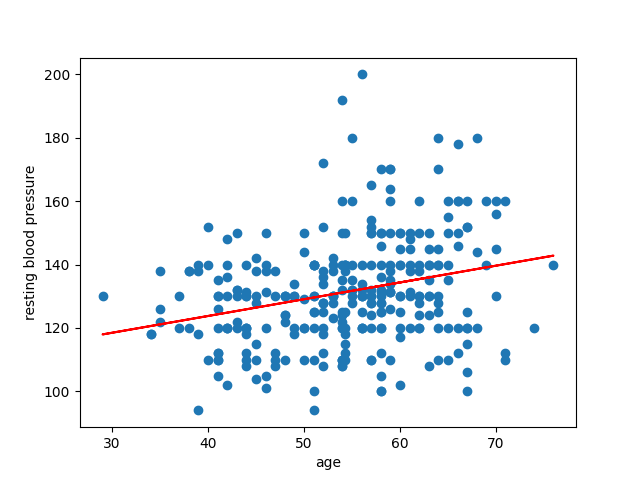
\includegraphics
                    [width=\textwidth,keepaspectratio]
                    {img/regression-5-Mean-imputation-resting-blood-pressure-age.png}
                    \caption
                    [regression-5-Mean-imputation-resting-blood-pressure-age]
                    {Współczynnik kierunkowy: 0.5289, Punkt przecięcia: 102.6334}
                    \label{regression-5-Mean-imputation-resting-blood-pressure-age}
                \end{figure}
                \FloatBarrier

                \begin{figure}[!htbp]
                    \centering
                    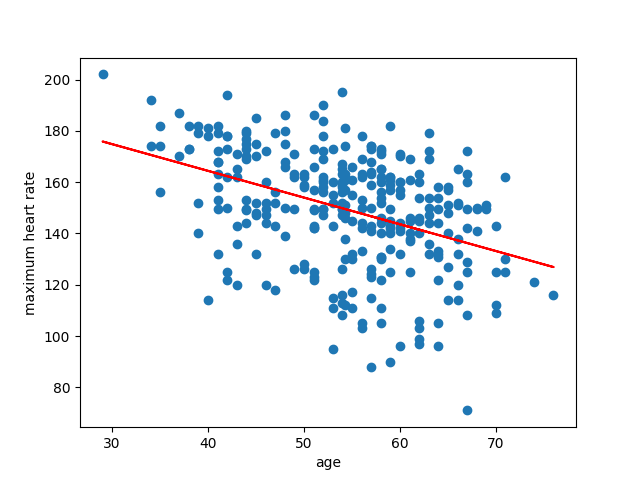
\includegraphics
                    [width=\textwidth,keepaspectratio]
                    {img/regression-5-Mean-imputation-maximum-heart-rate-age.png}
                    \caption
                    [regression-5-Mean-imputation-maximum-heart-rate-age]
                    {Współczynnik kierunkowy: -1.0417, Punkt przecięcia: 206.0584}
                    \label{regression-5-Mean-imputation-maximum-heart-rate-age}
                \end{figure}
                \FloatBarrier

            }

            \subsubsection{Interpolation}
            \label{results:5-percent:interpolation} {
                \begin{table}[!htbp]
                    \centering
                    \begin{tabular}{|c|c|c|c|c|c|c|}
                        \hline
                        & Mean & Std & Mode & Q1 & Median & Q3 \\ \hline
                        age & 54.2558 & 8.7904 & 58.0 & 48.0 & 55.0 & 60.0 \\ \hline
                        sex & 0.6733 & 0.4698 & 1.0 & 0.0 & 1.0 & 1.0 \\ \hline
                        chest-pain-type & 0.9802 & 1.0162 & 0.0 & 0.0 & 1.0 & 2.0 \\ \hline
                        resting-blood-pressure & 131.4818 & 17.2471 & 120.0 & 120.0 & 130.0 & 140.0 \\ \hline
                        serum-cholestoral & 246.3779 & 52.2324 & 234.0 & 211.0 & 240.0 & 275.1667 \\ \hline
                        fasting-blood-sugar & 0.132 & 0.3391 & 0.0 & 0.0 & 0.0 & 0.0 \\ \hline
                        resting-electrocardiographic & 0.5281 & 0.5259 & 1.0 & 0.0 & 1.0 & 1.0 \\ \hline
                        maximum-heart-rate & 149.7013 & 22.7039 & 162.0 & 136.0 & 153.0 & 165.5 \\ \hline
                        exercise-induced-angina & 0.3036 & 0.4606 & 0.0 & 0.0 & 0.0 & 1.0 \\ \hline
                        oldpeak & 1.021 & 1.1065 & 0.0 & 0.0 & 0.8 & 1.6 \\ \hline
                        the-slope-of-the-peak-exercise & 1.3993 & 0.6162 & 2.0 & 1.0 & 1.0 & 2.0 \\ \hline
                        number-of-major-vessels & 0.7294 & 0.9897 & 0.0 & 0.0 & 0.0 & 1.0 \\ \hline
                        thal & 2.2937 & 0.6004 & 2.0 & 2.0 & 2.0 & 3.0 \\ \hline
                        target & 0.5446 & 0.4988 & 1.0 & 0.0 & 1.0 & 1.0 \\ \hline
                    \end{tabular}
                    \caption{}
                    \label{result_5_Interpolation}
                \end{table}
                \FloatBarrier

                \begin{figure}[!htbp]
                    \centering
                    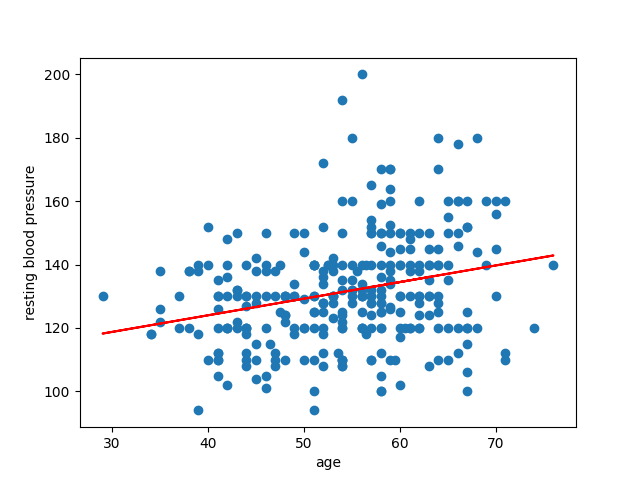
\includegraphics
                    [width=\textwidth,keepaspectratio]
                    {img/regression-5-Interpolation-resting-blood-pressure-age.png}
                    \caption
                    [regression-5-Interpolation-resting-blood-pressure-age]
                    {Współczynnik kierunkowy: 0.5243, Punkt przecięcia: 103.0352}
                    \label{regression-5-Interpolation-resting-blood-pressure-age}
                \end{figure}
                \FloatBarrier

                \begin{figure}[!htbp]
                    \centering
                    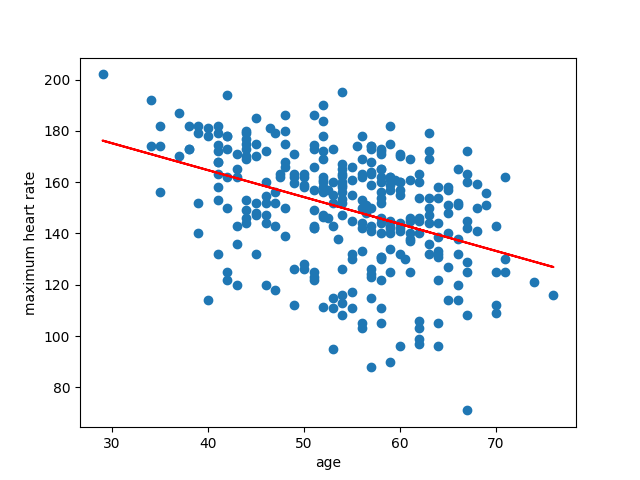
\includegraphics
                    [width=\textwidth,keepaspectratio]
                    {img/regression-5-Interpolation-maximum-heart-rate-age.png}
                    \caption
                    [regression-5-Interpolation-maximum-heart-rate-age]
                    {Współczynnik kierunkowy: -1.0493, Punkt przecięcia: 206.6338}
                    \label{regression-5-Interpolation-maximum-heart-rate-age}
                \end{figure}
                \FloatBarrier

            }

            \subsubsection{Hot deck}
            \label{results:5-percent:dot-deck} {
                \begin{table}[!htbp]
                    \centering
                    \begin{tabular}{|c|c|c|c|c|c|c|}
                        \hline
                        & Mean & Std & Mode & Q1 & Median & Q3 \\ \hline
                        age & 54.5215 & 8.8182 & 59.0 & 48.0 & 56.0 & 60.5 \\ \hline
                        sex & 0.6931 & 0.462 & 1.0 & 0.0 & 1.0 & 1.0 \\ \hline
                        chest-pain-type & 0.9901 & 1.018 & 0.0 & 0.0 & 1.0 & 2.0 \\ \hline
                        resting-blood-pressure & 131.429 & 17.1287 & 130.0 & 120.0 & 130.0 & 140.0 \\ \hline
                        serum-cholestoral & 245.0792 & 54.0866 & 234.0 & 207.5 & 236.0 & 274.0 \\ \hline
                        fasting-blood-sugar & 0.1353 & 0.3426 & 0.0 & 0.0 & 0.0 & 0.0 \\ \hline
                        resting-electrocardiographic & 0.5479 & 0.5244 & 1.0 & 0.0 & 1.0 & 1.0 \\ \hline
                        maximum-heart-rate & 149.4884 & 23.1365 & 162.0 & 133.5 & 153.0 & 166.0 \\ \hline
                        exercise-induced-angina & 0.3399 & 0.4745 & 0.0 & 0.0 & 0.0 & 1.0 \\ \hline
                        oldpeak & 0.9954 & 1.1182 & 0.0 & 0.0 & 0.6 & 1.6 \\ \hline
                        the-slope-of-the-peak-exercise & 1.4125 & 0.6074 & 2.0 & 1.0 & 1.0 & 2.0 \\ \hline
                        number-of-major-vessels & 0.6733 & 1.0011 & 0.0 & 0.0 & 0.0 & 1.0 \\ \hline
                        thal & 2.2937 & 0.5948 & 2.0 & 2.0 & 2.0 & 3.0 \\ \hline
                        target & 0.5611 & 0.4971 & 1.0 & 0.0 & 1.0 & 1.0 \\ \hline
                    \end{tabular}
                    \caption{}
                    \label{result_5_Hot-deck}
                \end{table}
                \FloatBarrier

                \begin{figure}[!htbp]
                    \centering
                    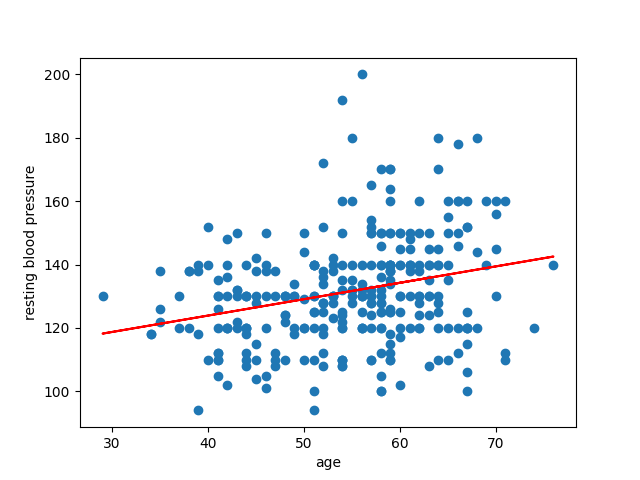
\includegraphics
                    [width=\textwidth,keepaspectratio]
                    {img/regression-5-Hot-deck-resting-blood-pressure-age.png}
                    \caption
                    [regression-5-Hot-deck-resting-blood-pressure-age]
                    {Współczynnik kierunkowy: 0.5173, Punkt przecięcia: 103.2271}
                    \label{regression-5-Hot-deck-resting-blood-pressure-age}
                \end{figure}
                \FloatBarrier

                \begin{figure}[!htbp]
                    \centering
                    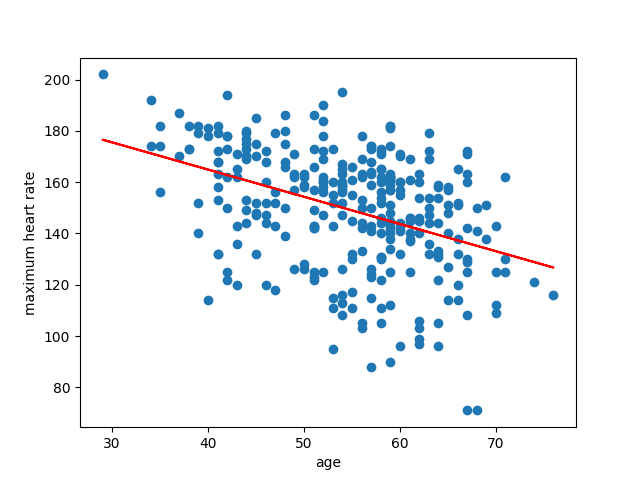
\includegraphics
                    [width=\textwidth,keepaspectratio]
                    {img/regression-5-Hot-deck-maximum-heart-rate-age.png}
                    \caption
                    [regression-5-Hot-deck-maximum-heart-rate-age]
                    {Współczynnik kierunkowy: -1.0607, Punkt przecięcia: 207.3196}
                    \label{regression-5-Hot-deck-maximum-heart-rate-age}
                \end{figure}
                \FloatBarrier

            }

            \subsubsection{Regression}
            \label{results:5-percent:regression} {
                \begin{table}[!htbp]
                    \centering
                    \begin{tabular}{|c|c|c|c|c|c|c|}
                        \hline
                        & Mean & Std & Mode & Q1 & Median & Q3 \\ \hline
                        age & 54.1981 & 8.7838 & 58.0 & 48.0 & 55.0 & 60.0 \\ \hline
                        sex & 0.6799 & 0.4673 & 1.0 & 0.0 & 1.0 & 1.0 \\ \hline
                        chest-pain-type & 1.0297 & 1.0305 & 0.0 & 0.0 & 1.0 & 2.0 \\ \hline
                        resting-blood-pressure & 131.3432 & 17.1124 & 120.0 & 120.0 & 130.0 & 140.0 \\ \hline
                        serum-cholestoral & 246.0021 & 51.3759 & 197.0 & 211.5 & 240.0 & 274.0 \\ \hline
                        fasting-blood-sugar & 0.132 & 0.3391 & 0.0 & 0.0 & 0.0 & 0.0 \\ \hline
                        resting-electrocardiographic & 0.5479 & 0.5244 & 1.0 & 0.0 & 1.0 & 1.0 \\ \hline
                        maximum-heart-rate & 149.9182 & 22.6091 & 162.0 & 136.5 & 153.0 & 166.0 \\ \hline
                        exercise-induced-angina & 0.3036 & 0.4606 & 0.0 & 0.0 & 0.0 & 1.0 \\ \hline
                        oldpeak & 1.0201 & 1.1124 & 0.0 & 0.0 & 0.8 & 1.6 \\ \hline
                        the-slope-of-the-peak-exercise & 1.4059 & 0.6119 & 2.0 & 1.0 & 1.0 & 2.0 \\ \hline
                        number-of-major-vessels & 0.6337 & 0.9635 & 0.0 & 0.0 & 0.0 & 1.0 \\ \hline
                        thal & 2.2871 & 0.5869 & 2.0 & 2.0 & 2.0 & 3.0 \\ \hline
                        target & 0.5644 & 0.4967 & 1.0 & 0.0 & 1.0 & 1.0 \\ \hline
                    \end{tabular}
                    \caption{}
                    \label{result_5_Regression}
                \end{table}
                \FloatBarrier

                \begin{figure}[!htbp]
                    \centering
                    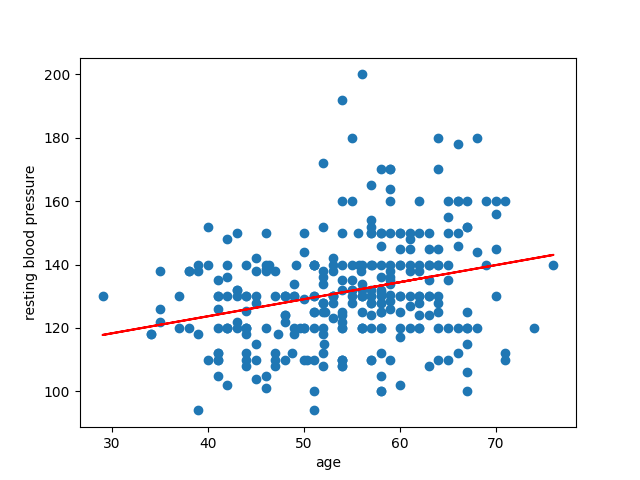
\includegraphics
                    [width=\textwidth,keepaspectratio]
                    {img/regression-5-Regression-resting-blood-pressure-age.png}
                    \caption
                    [regression-5-Regression-resting-blood-pressure-age]
                    {Współczynnik kierunkowy: 0.5377, Punkt przecięcia: 102.2009}
                    \label{regression-5-Regression-resting-blood-pressure-age}
                \end{figure}
                \FloatBarrier

                \begin{figure}[!htbp]
                    \centering
                    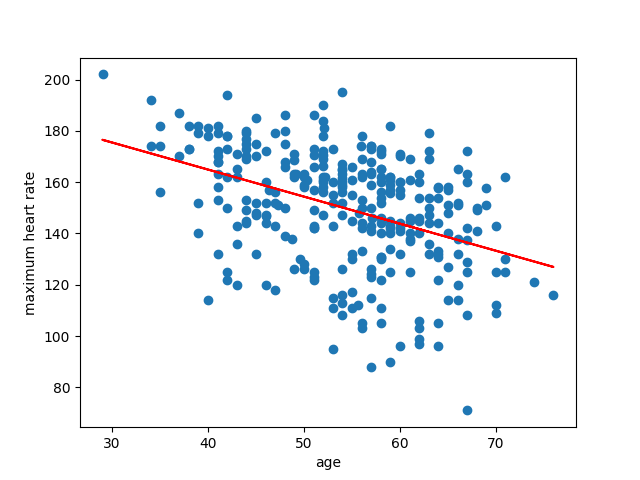
\includegraphics
                    [width=\textwidth,keepaspectratio]
                    {img/regression-5-Regression-maximum-heart-rate-age.png}
                    \caption
                    [regression-5-Regression-maximum-heart-rate-age]
                    {Współczynnik kierunkowy: -1.0547, Punkt przecięcia: 207.0784}
                    \label{regression-5-Regression-maximum-heart-rate-age}
                \end{figure}
                \FloatBarrier

            }
        }
        \newpage

        \subsection{Braki w danych 15\%}
        \label{results:15-percent} {

            \subsubsection{List wise deletion}
            \label{results:15-percent:list-wise} {
                \begin{table}[!htbp]
                    \centering
                    \begin{tabular}{|c|c|c|c|c|c|c|}
                        \hline
                        & Mean & Std & Mode & Q1 & Median & Q3 \\ \hline
                        age & 52.0 & 7.1487 & 52.0 & 49.0 & 52.0 & 55.5 \\ \hline
                        sex & 0.7667 & 0.4302 & 1.0 & 1.0 & 1.0 & 1.0 \\ \hline
                        chest-pain-type & 1.3 & 1.1188 & 2.0 & 0.0 & 2.0 & 2.0 \\ \hline
                        resting-blood-pressure & 127.7 & 12.0977 & 120.0 & 118.5 & 126.5 & 138.0 \\ \hline
                        serum-cholestoral & 241.3333 & 46.9588 & 197.0 & 203.5 & 237.5 & 275.25 \\ \hline
                        fasting-blood-sugar & 0.1 & 0.3051 & 0.0 & 0.0 & 0.0 & 0.0 \\ \hline
                        resting-electrocardiographic & 0.5 & 0.5724 & 0.0 & 0.0 & 0.0 & 1.0 \\ \hline
                        maximum-heart-rate & 158.9 & 19.9937 & 152.0 & 151.25 & 161.5 & 173.5 \\ \hline
                        exercise-induced-angina & 0.2667 & 0.4498 & 0.0 & 0.0 & 0.0 & 0.75 \\ \hline
                        oldpeak & 0.83 & 1.0577 & 0.0 & 0.0 & 0.55 & 1.2 \\ \hline
                        the-slope-of-the-peak-exercise & 1.3333 & 0.7112 & 2.0 & 1.0 & 1.0 & 2.0 \\ \hline
                        number-of-major-vessels & 0.6333 & 1.0981 & 0.0 & 0.0 & 0.0 & 1.0 \\ \hline
                        thal & 2.2333 & 0.6261 & 2.0 & 2.0 & 2.0 & 3.0 \\ \hline
                        target & 0.7333 & 0.4498 & 1.0 & 0.25 & 1.0 & 1.0 \\ \hline
                    \end{tabular}
                    \caption{}
                    \label{result_15_List-wise-deletion}
                \end{table}
                \FloatBarrier

                \begin{figure}[!htbp]
                    \centering
                    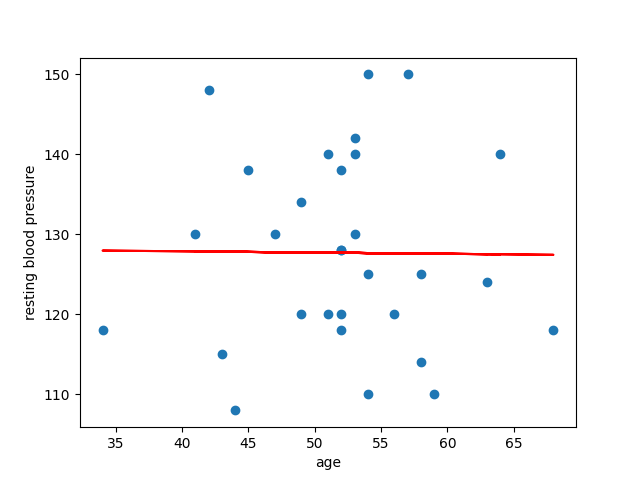
\includegraphics
                    [width=\textwidth,keepaspectratio]
                    {img/regression-15-List-wise-deletion-resting-blood-pressure-age.png}
                    \caption
                    [regression-15-List-wise-deletion-resting-blood-pressure-age]
                    {Współczynnik kierunkowy: -0.0155, Punkt przecięcia: 128.507}
                    \label{regression-15-List-wise-deletion-resting-blood-pressure-age}
                \end{figure}
                \FloatBarrier

                \begin{figure}[!htbp]
                    \centering
                    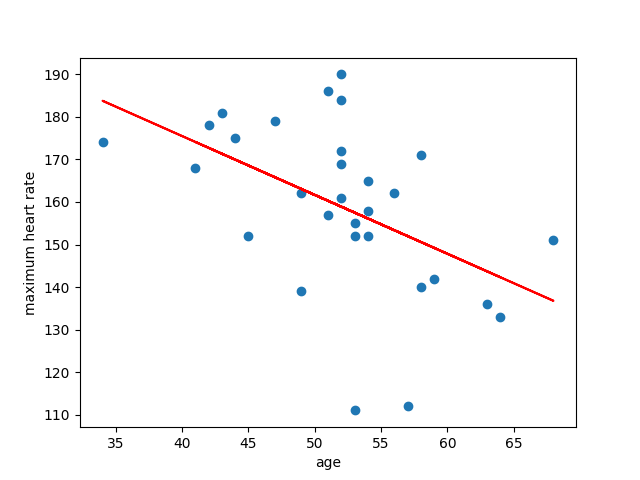
\includegraphics
                    [width=\textwidth,keepaspectratio]
                    {img/regression-15-List-wise-deletion-maximum-heart-rate-age.png}
                    \caption
                    [regression-15-List-wise-deletion-maximum-heart-rate-age]
                    {Współczynnik kierunkowy: -1.3833, Punkt przecięcia: 230.8298}
                    \label{regression-15-List-wise-deletion-maximum-heart-rate-age}
                \end{figure}
                \FloatBarrier

            }

            \subsubsection{Mean imputation}
            \label{results:15-percent:mean-input} {
                \begin{table}[!htbp]
                    \centering
                    \begin{tabular}{|c|c|c|c|c|c|c|}
                        \hline
                        & Mean & Std & Mode & Q1 & Median & Q3 \\ \hline
                        age & 54.1712 & 8.3071 & 54.1712 & 49.5 & 54.1712 & 59.5 \\ \hline
                        sex & 0.7261 & 0.4467 & 1.0 & 0.0 & 1.0 & 1.0 \\ \hline
                        chest-pain-type & 0.9835 & 0.9576 & 0.0 & 0.0 & 1.0 & 2.0 \\ \hline
                        resting-blood-pressure & 131.4318 & 16.546 & 131.4318 & 120.0 & 131.4318 & 140.0 \\ \hline
                        serum-cholestoral & 247.3472 & 49.3824 & 247.3472 & 214.0 & 247.3472 & 269.0 \\ \hline
                        fasting-blood-sugar & 0.1254 & 0.3317 & 0.0 & 0.0 & 0.0 & 0.0 \\ \hline
                        resting-electrocardiographic & 0.604 & 0.5162 & 1.0 & 0.0 & 1.0 & 1.0 \\ \hline
                        maximum-heart-rate & 151.1875 & 20.5691 & 151.1875 & 143.0 & 151.1875 & 163.0 \\ \hline
                        exercise-induced-angina & 0.2838 & 0.4516 & 0.0 & 0.0 & 0.0 & 1.0 \\ \hline
                        oldpeak & 1.0402 & 1.0868 & 0.0 & 0.0 & 1.0 & 1.5 \\ \hline
                        the-slope-of-the-peak-exercise & 1.3333 & 0.5849 & 1.0 & 1.0 & 1.0 & 2.0 \\ \hline
                        number-of-major-vessels & 0.7723 & 0.9513 & 0.0 & 0.0 & 1.0 & 1.0 \\ \hline
                        thal & 2.2739 & 0.5819 & 2.0 & 2.0 & 2.0 & 3.0 \\ \hline
                        target & 0.6007 & 0.4906 & 1.0 & 0.0 & 1.0 & 1.0 \\ \hline
                    \end{tabular}
                    \caption{}
                    \label{result_15_Mean-imputation}
                \end{table}
                \FloatBarrier

                \begin{figure}[!htbp]
                    \centering
                    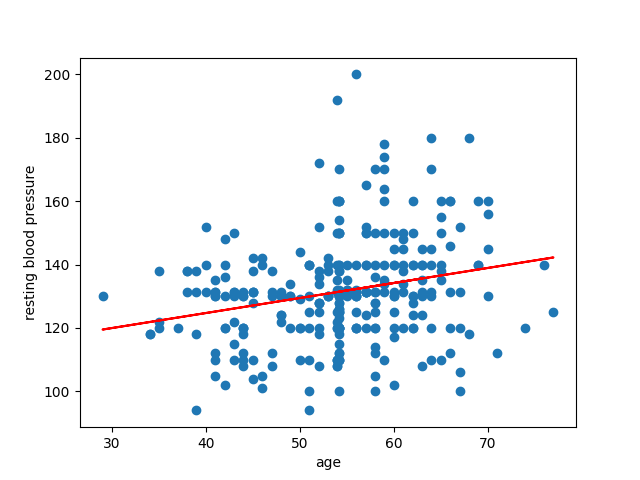
\includegraphics
                    [width=\textwidth,keepaspectratio]
                    {img/regression-15-Mean-imputation-resting-blood-pressure-age.png}
                    \caption
                    [regression-15-Mean-imputation-resting-blood-pressure-age]
                    {Współczynnik kierunkowy: 0.4738, Punkt przecięcia: 105.7662}
                    \label{regression-15-Mean-imputation-resting-blood-pressure-age}
                \end{figure}
                \FloatBarrier

                \begin{figure}[!htbp]
                    \centering
                    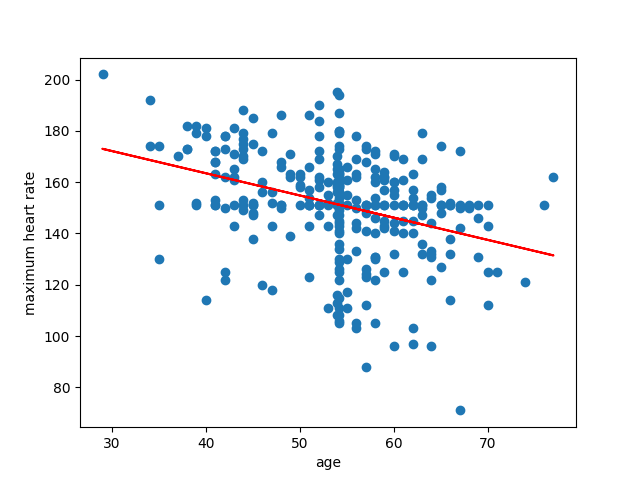
\includegraphics
                    [width=\textwidth,keepaspectratio]
                    {img/regression-15-Mean-imputation-maximum-heart-rate-age.png}
                    \caption
                    [regression-15-Mean-imputation-maximum-heart-rate-age]
                    {Współczynnik kierunkowy: -0.8659, Punkt przecięcia: 198.0939}
                    \label{regression-15-Mean-imputation-maximum-heart-rate-age}
                \end{figure}
                \FloatBarrier

            }

            \subsubsection{Interpolation}
            \label{results:15-percent:interpolation} {
                \begin{table}[!htbp]
                    \centering
                    \begin{tabular}{|c|c|c|c|c|c|c|}
                        \hline
                        & Mean & Std & Mode & Q1 & Median & Q3 \\ \hline
                        age & 54.0513 & 8.6269 & 54.0 & 48.0 & 55.0 & 60.0 \\ \hline
                        sex & 0.649 & 0.4781 & 1.0 & 0.0 & 1.0 & 1.0 \\ \hline
                        chest-pain-type & 0.9437 & 1.005 & 0.0 & 0.0 & 1.0 & 2.0 \\ \hline
                        resting-blood-pressure & 131.1904 & 16.9762 & 120.0 & 120.0 & 130.0 & 140.0 \\ \hline
                        serum-cholestoral & 246.6838 & 50.543 & 197.0 & 212.0 & 242.5 & 272.5 \\ \hline
                        fasting-blood-sugar & 0.1258 & 0.3322 & 0.0 & 0.0 & 0.0 & 0.0 \\ \hline
                        resting-electrocardiographic & 0.5166 & 0.5264 & 0.0 & 0.0 & 1.0 & 1.0 \\ \hline
                        maximum-heart-rate & 150.7897 & 21.6155 & 162.0 & 138.25 & 154.0 & 165.875 \\ \hline
                        exercise-induced-angina & 0.3311 & 0.4714 & 0.0 & 0.0 & 0.0 & 1.0 \\ \hline
                        oldpeak & 1.0257 & 1.1411 & 0.0 & 0.0 & 0.7417 & 1.6 \\ \hline
                        the-slope-of-the-peak-exercise & 1.3411 & 0.6096 & 1.0 & 1.0 & 1.0 & 2.0 \\ \hline
                        number-of-major-vessels & 0.702 & 0.9903 & 0.0 & 0.0 & 0.0 & 1.0 \\ \hline
                        thal & 2.3212 & 0.6041 & 2.0 & 2.0 & 2.0 & 3.0 \\ \hline
                        target & 0.543 & 0.499 & 1.0 & 0.0 & 1.0 & 1.0 \\ \hline
                    \end{tabular}
                    \caption{}
                    \label{result_15_Interpolation}
                \end{table}
                \FloatBarrier

                \begin{figure}[!htbp]
                    \centering
                    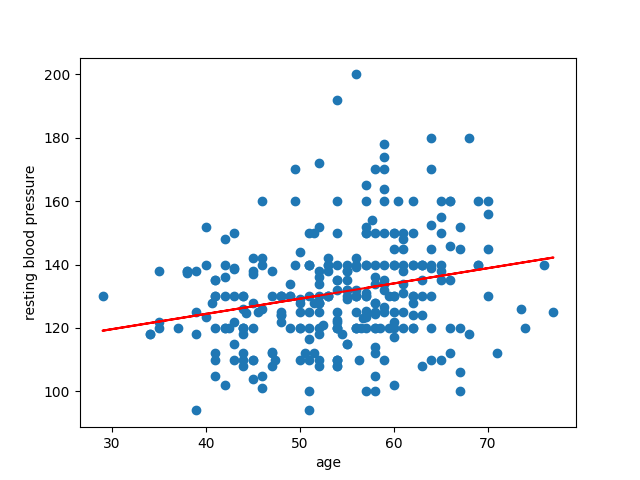
\includegraphics
                    [width=\textwidth,keepaspectratio]
                    {img/regression-15-Interpolation-resting-blood-pressure-age.png}
                    \caption
                    [regression-15-Interpolation-resting-blood-pressure-age]
                    {Współczynnik kierunkowy: 0.4809, Punkt przecięcia: 105.1974}
                    \label{regression-15-Interpolation-resting-blood-pressure-age}
                \end{figure}
                \FloatBarrier

                \begin{figure}[!htbp]
                    \centering
                    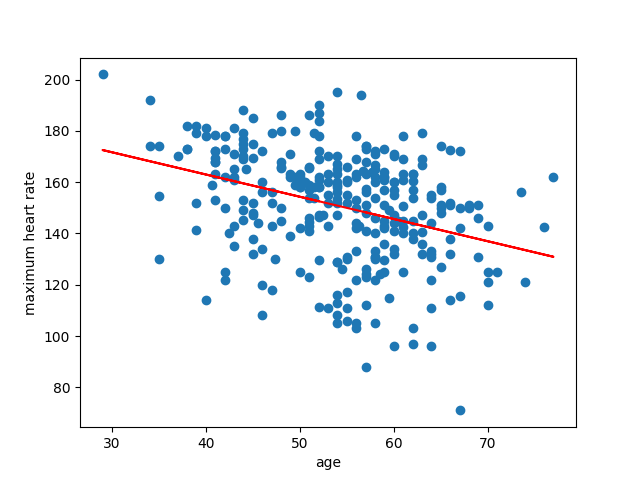
\includegraphics
                    [width=\textwidth,keepaspectratio]
                    {img/regression-15-Interpolation-maximum-heart-rate-age.png}
                    \caption
                    [regression-15-Interpolation-maximum-heart-rate-age]
                    {Współczynnik kierunkowy: -0.8672, Punkt przecięcia: 197.6622}
                    \label{regression-15-Interpolation-maximum-heart-rate-age}
                \end{figure}
                \FloatBarrier

            }

            \subsubsection{Hot deck}
            \label{results:15-percent:dot-deck} {
                \begin{table}[!htbp]
                    \centering
                    \begin{tabular}{|c|c|c|c|c|c|c|}
                        \hline
                        & Mean & Std & Mode & Q1 & Median & Q3 \\ \hline
                        age & 53.7657 & 8.911 & 57.0 & 46.0 & 56.0 & 60.0 \\ \hline
                        sex & 0.7063 & 0.4562 & 1.0 & 0.0 & 1.0 & 1.0 \\ \hline
                        chest-pain-type & 0.9208 & 1.0133 & 0.0 & 0.0 & 1.0 & 2.0 \\ \hline
                        resting-blood-pressure & 131.6469 & 17.1218 & 130.0 & 120.0 & 130.0 & 140.0 \\ \hline
                        serum-cholestoral & 249.4389 & 51.0181 & 271.0 & 213.0 & 247.0 & 273.0 \\ \hline
                        fasting-blood-sugar & 0.1353 & 0.3426 & 0.0 & 0.0 & 0.0 & 0.0 \\ \hline
                        resting-electrocardiographic & 0.5479 & 0.5244 & 1.0 & 0.0 & 1.0 & 1.0 \\ \hline
                        maximum-heart-rate & 149.6535 & 22.9885 & 141.0 & 137.0 & 153.0 & 166.0 \\ \hline
                        exercise-induced-angina & 0.3399 & 0.4745 & 0.0 & 0.0 & 0.0 & 1.0 \\ \hline
                        oldpeak & 1.033 & 1.1596 & 0.0 & 0.0 & 0.8 & 1.6 \\ \hline
                        the-slope-of-the-peak-exercise & 1.4125 & 0.6074 & 2.0 & 1.0 & 1.0 & 2.0 \\ \hline
                        number-of-major-vessels & 0.7855 & 1.0627 & 0.0 & 0.0 & 0.0 & 1.0 \\ \hline
                        thal & 2.33 & 0.6171 & 2.0 & 2.0 & 2.0 & 3.0 \\ \hline
                        target & 0.5248 & 0.5002 & 1.0 & 0.0 & 1.0 & 1.0 \\ \hline
                    \end{tabular}
                    \caption{}
                    \label{result_15_Hot-deck}
                \end{table}
                \FloatBarrier

                \begin{figure}[!htbp]
                    \centering
                    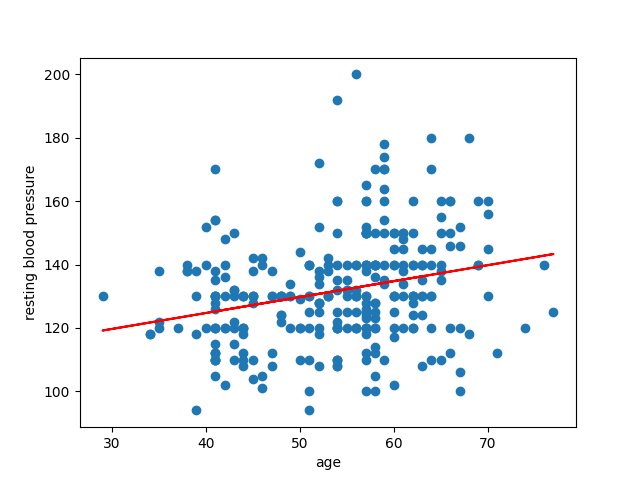
\includegraphics
                    [width=\textwidth,keepaspectratio]
                    {img/regression-15-Hot-deck-resting-blood-pressure-age.png}
                    \caption
                    [regression-15-Hot-deck-resting-blood-pressure-age]
                    {Współczynnik kierunkowy: 0.5028, Punkt przecięcia: 104.6144}
                    \label{regression-15-Hot-deck-resting-blood-pressure-age}
                \end{figure}
                \FloatBarrier

                \begin{figure}[!htbp]
                    \centering
                    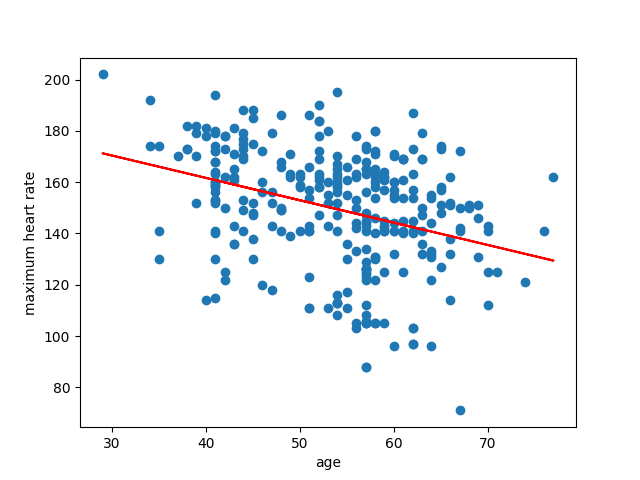
\includegraphics
                    [width=\textwidth,keepaspectratio]
                    {img/regression-15-Hot-deck-maximum-heart-rate-age.png}
                    \caption
                    [regression-15-Hot-deck-maximum-heart-rate-age]
                    {Współczynnik kierunkowy: -0.8717, Punkt przecięcia: 196.5231}
                    \label{regression-15-Hot-deck-maximum-heart-rate-age}
                \end{figure}
                \FloatBarrier

            }

            \subsubsection{Regression}
            \label{results:15-percent:regression} {
                \begin{table}[!htbp]
                    \centering
                    \begin{tabular}{|c|c|c|c|c|c|c|}
                        \hline
                        & Mean & Std & Mode & Q1 & Median & Q3 \\ \hline
                        age & 53.714 & 8.6974 & 54.0 & 47.0 & 54.0 & 60.0 \\ \hline
                        sex & 0.6964 & 0.4606 & 1.0 & 0.0 & 1.0 & 1.0 \\ \hline
                        chest-pain-type & 1.0528 & 1.0248 & 0.0 & 0.0 & 1.0 & 2.0 \\ \hline
                        resting-blood-pressure & 131.1375 & 17.0185 & 120.0 & 120.0 & 130.0 & 140.0 \\ \hline
                        serum-cholestoral & 247.0421 & 51.2247 & 197.0 & 211.7721 & 243.0 & 277.0 \\ \hline
                        fasting-blood-sugar & 0.1254 & 0.3317 & 0.0 & 0.0 & 0.0 & 0.0 \\ \hline
                        resting-electrocardiographic & 0.505 & 0.5266 & 0.0 & 0.0 & 0.0 & 1.0 \\ \hline
                        maximum-heart-rate & 152.3587 & 21.0286 & 162.0 & 143.0 & 156.0 & 166.0 \\ \hline
                        exercise-induced-angina & 0.2937 & 0.4562 & 0.0 & 0.0 & 0.0 & 1.0 \\ \hline
                        oldpeak & 1.0149 & 1.1179 & 0.0 & 0.0 & 0.7295 & 1.6 \\ \hline
                        the-slope-of-the-peak-exercise & 1.4653 & 0.6181 & 2.0 & 1.0 & 2.0 & 2.0 \\ \hline
                        number-of-major-vessels & 0.6139 & 0.983 & 0.0 & 0.0 & 0.0 & 1.0 \\ \hline
                        thal & 2.2739 & 0.5819 & 2.0 & 2.0 & 2.0 & 3.0 \\ \hline
                        target & 0.5842 & 0.4937 & 1.0 & 0.0 & 1.0 & 1.0 \\ \hline
                    \end{tabular}
                    \caption{}
                    \label{result_15_Regression}
                \end{table}
                \FloatBarrier

                \begin{figure}[!htbp]
                    \centering
                    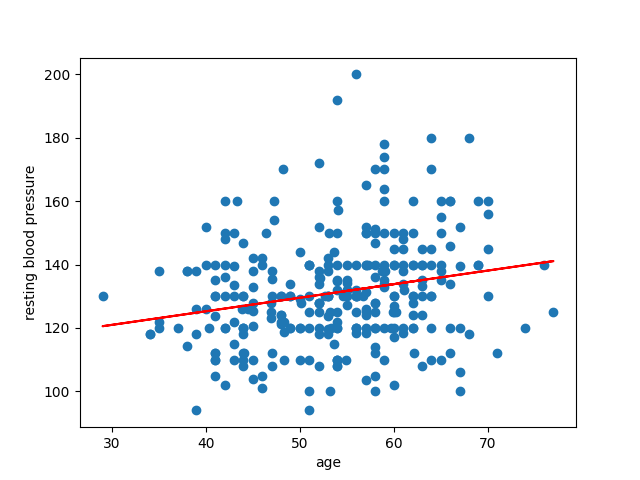
\includegraphics
                    [width=\textwidth,keepaspectratio]
                    {img/regression-15-Regression-resting-blood-pressure-age.png}
                    \caption
                    [regression-15-Regression-resting-blood-pressure-age]
                    {Współczynnik kierunkowy: 0.4281, Punkt przecięcia: 108.1442}
                    \label{regression-15-Regression-resting-blood-pressure-age}
                \end{figure}
                \FloatBarrier

                \begin{figure}[!htbp]
                    \centering
                    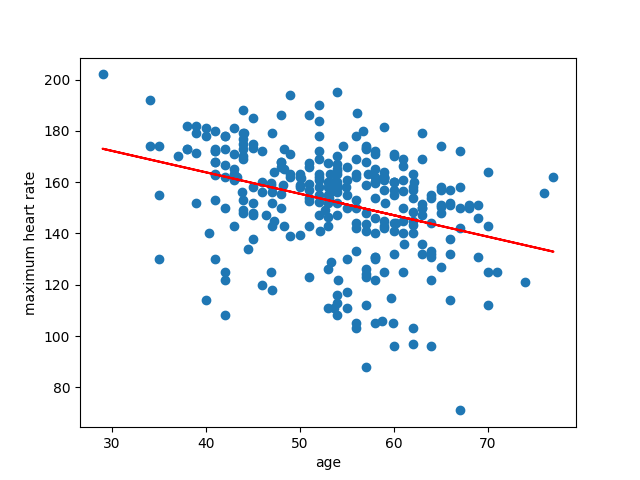
\includegraphics
                    [width=\textwidth,keepaspectratio]
                    {img/regression-15-Regression-maximum-heart-rate-age.png}
                    \caption
                    [regression-15-Regression-maximum-heart-rate-age]
                    {Współczynnik kierunkowy: -0.8362, Punkt przecięcia: 197.2746}
                    \label{regression-15-Regression-maximum-heart-rate-age}
                \end{figure}
                \FloatBarrier

            }
        }
        \newpage

        \subsection{Braki w danych 30\%}
        \label{results:30-percent} {

            \subsubsection{List wise deletion}
            \label{results:30-percent:list-wise} {

                \begin{table}[!htbp]
                    \centering
                    \begin{tabular}{|c|c|c|c|c|c|c|}
                        \hline
                        & Mean & Std & Mode & Q1 & Median & Q3 \\ \hline
                        age & 46.5 & 6.364 & 42.0 & 44.25 & 46.5 & 48.75 \\ \hline
                        sex & 0.5 & 0.7071 & 0.0 & 0.25 & 0.5 & 0.75 \\ \hline
                        chest-pain-type & 1.0 & 1.4142 & 0.0 & 0.5 & 1.0 & 1.5 \\ \hline
                        resting-blood-pressure & 98.0 & 5.6569 & 94.0 & 96.0 & 98.0 & 100.0 \\ \hline
                        serum-cholestoral & 246.0 & 26.8701 & 227.0 & 236.5 & 246.0 & 255.5 \\ \hline
                        fasting-blood-sugar & 0.0 & 0.0 & 0.0 & 0.0 & 0.0 & 0.0 \\ \hline
                        resting-electrocardiographic & 0.5 & 0.7071 & 0.0 & 0.25 & 0.5 & 0.75 \\ \hline
                        maximum-heart-rate & 138.0 & 22.6274 & 122.0 & 130.0 & 138.0 & 146.0 \\ \hline
                        exercise-induced-angina & 0.5 & 0.7071 & 0.0 & 0.25 & 0.5 & 0.75 \\ \hline
                        oldpeak & 0.3 & 0.4243 & 0.0 & 0.15 & 0.3 & 0.45 \\ \hline
                        the-slope-of-the-peak-exercise & 1.5 & 0.7071 & 1.0 & 1.25 & 1.5 & 1.75 \\ \hline
                        number-of-major-vessels & 0.5 & 0.7071 & 0.0 & 0.25 & 0.5 & 0.75 \\ \hline
                        thal & 2.5 & 0.7071 & 2.0 & 2.25 & 2.5 & 2.75 \\ \hline
                        target & 1.0 & 0.0 & 1.0 & 1.0 & 1.0 & 1.0 \\ \hline
                    \end{tabular}
                    \caption{}
                    \label{result_30_List-wise-deletion}
                \end{table}
                \FloatBarrier

                \begin{figure}[!htbp]
                    \centering
                    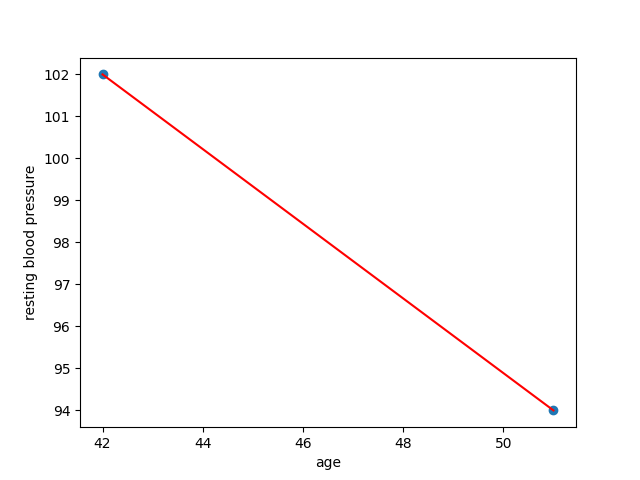
\includegraphics
                    [width=\textwidth,keepaspectratio]
                    {img/regression-30-List-wise-deletion-resting-blood-pressure-age.png}
                    \caption
                    [regression-30-List-wise-deletion-resting-blood-pressure-age]
                    {Współczynnik kierunkowy: -0.8889, Punkt przecięcia: 139.3333}
                    \label{regression-30-List-wise-deletion-resting-blood-pressure-age}
                \end{figure}
                \FloatBarrier

                \begin{figure}[!htbp]
                    \centering
                    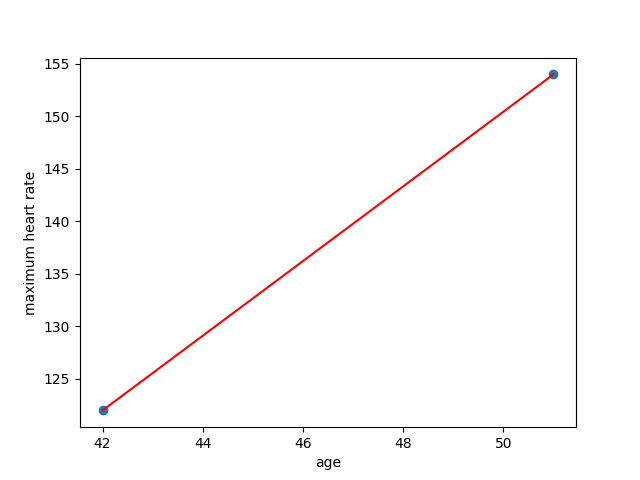
\includegraphics
                    [width=\textwidth,keepaspectratio]
                    {img/regression-30-List-wise-deletion-maximum-heart-rate-age.png}
                    \caption
                    [regression-30-List-wise-deletion-maximum-heart-rate-age]
                    {Współczynnik kierunkowy: 3.5556, Punkt przecięcia: -27.3333}
                    \label{regression-30-List-wise-deletion-maximum-heart-rate-age}
                \end{figure}
                \FloatBarrier
            }

            \subsubsection{Mean imputation}
            \label{results:30-percent:mean-input} {
                \begin{table}[!htbp]
                    \centering
                    \begin{tabular}{|c|c|c|c|c|c|c|}
                        \hline
                        & Mean & Std & Mode & Q1 & Median & Q3 \\ \hline
                        age & 54.2755 & 7.4138 & 54.2755 & 52.0 & 54.2755 & 58.0 \\ \hline
                        sex & 0.7921 & 0.4065 & 1.0 & 1.0 & 1.0 & 1.0 \\ \hline
                        chest-pain-type & 0.9736 & 0.8608 & 1.0 & 0.0 & 1.0 & 1.0 \\ \hline
                        resting-blood-pressure & 130.5311 & 13.982 & 130.5311 & 124.0 & 130.5311 & 134.0 \\ \hline
                        serum-cholestoral & 246.1991 & 40.5367 & 246.1991 & 225.5 & 246.1991 & 260.0 \\ \hline
                        fasting-blood-sugar & 0.1122 & 0.3161 & 0.0 & 0.0 & 0.0 & 0.0 \\ \hline
                        resting-electrocardiographic & 0.6535 & 0.4971 & 1.0 & 0.0 & 1.0 & 1.0 \\ \hline
                        maximum-heart-rate & 149.8873 & 18.8264 & 149.8873 & 144.0 & 149.8873 & 160.0 \\ \hline
                        exercise-induced-angina & 0.2112 & 0.4089 & 0.0 & 0.0 & 0.0 & 0.0 \\ \hline
                        oldpeak & 1.0326 & 0.9452 & 1.0326 & 0.2 & 1.0326 & 1.2 \\ \hline
                        the-slope-of-the-peak-exercise & 1.297 & 0.5733 & 1.0 & 1.0 & 1.0 & 2.0 \\ \hline
                        number-of-major-vessels & 0.8119 & 0.8808 & 1.0 & 0.0 & 1.0 & 1.0 \\ \hline
                        thal & 2.2442 & 0.5396 & 2.0 & 2.0 & 2.0 & 3.0 \\ \hline
                        target & 0.7063 & 0.4562 & 1.0 & 0.0 & 1.0 & 1.0 \\ \hline
                    \end{tabular}
                    \caption{}
                    \label{result_30_Mean-imputation}
                \end{table}
                \FloatBarrier

                \begin{figure}[!htbp]
                    \centering
                    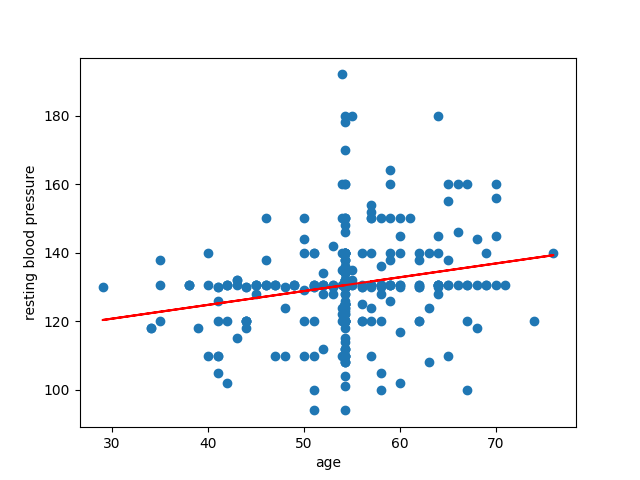
\includegraphics
                    [width=\textwidth,keepaspectratio]
                    {img/regression-30-Mean-imputation-resting-blood-pressure-age.png}
                    \caption
                    [regression-30-Mean-imputation-resting-blood-pressure-age]
                    {Współczynnik kierunkowy: 0.4026, Punkt przecięcia: 108.6808}
                    \label{regression-30-Mean-imputation-resting-blood-pressure-age}
                \end{figure}
                \FloatBarrier

                \begin{figure}[!htbp]
                    \centering
                    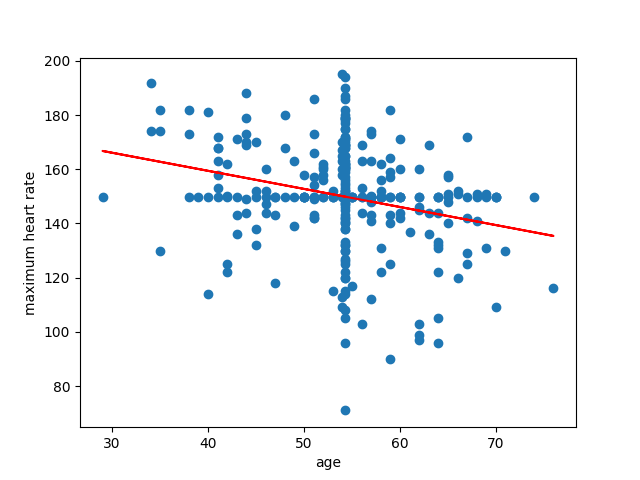
\includegraphics
                    [width=\textwidth,keepaspectratio]
                    {img/regression-30-Mean-imputation-maximum-heart-rate-age.png}
                    \caption
                    [regression-30-Mean-imputation-maximum-heart-rate-age]
                    {Współczynnik kierunkowy: -0.6673, Punkt przecięcia: 186.1078}
                    \label{regression-30-Mean-imputation-maximum-heart-rate-age}
                \end{figure}
                \FloatBarrier

            }

            \subsubsection{Interpolation}
            \label{results:30-percent:interpolation} {
                \begin{table}[!htbp]
                    \centering
                    \begin{tabular}{|c|c|c|c|c|c|c|}
                        \hline
                        & Mean & Std & Mode & Q1 & Median & Q3 \\ \hline
                        age & 54.1204 & 8.3722 & 57.0 & 48.0 & 54.0 & 60.0 \\ \hline
                        sex & 0.6421 & 0.4802 & 1.0 & 0.0 & 1.0 & 1.0 \\ \hline
                        chest-pain-type & 0.913 & 0.9336 & 0.0 & 0.0 & 1.0 & 2.0 \\ \hline
                        resting-blood-pressure & 130.9649 & 15.7225 & 130.0 & 120.0 & 130.0 & 140.0 \\ \hline
                        serum-cholestoral & 244.3595 & 44.8516 & 197.0 & 212.25 & 241.5 & 269.5 \\ \hline
                        fasting-blood-sugar & 0.1371 & 0.3446 & 0.0 & 0.0 & 0.0 & 0.0 \\ \hline
                        resting-electrocardiographic & 0.5251 & 0.5327 & 0.0 & 0.0 & 1.0 & 1.0 \\ \hline
                        maximum-heart-rate & 149.1538 & 21.3123 & 152.0 & 138.0 & 152.0 & 165.0 \\ \hline
                        exercise-induced-angina & 0.301 & 0.4595 & 0.0 & 0.0 & 0.0 & 1.0 \\ \hline
                        oldpeak & 1.0258 & 1.0343 & 0.0 & 0.1 & 0.8 & 1.67 \\ \hline
                        the-slope-of-the-peak-exercise & 1.3579 & 0.6095 & 1.0 & 1.0 & 1.0 & 2.0 \\ \hline
                        number-of-major-vessels & 0.689 & 0.9695 & 0.0 & 0.0 & 0.0 & 1.0 \\ \hline
                        thal & 2.3211 & 0.5827 & 2.0 & 2.0 & 2.0 & 3.0 \\ \hline
                        target & 0.5351 & 0.4996 & 1.0 & 0.0 & 1.0 & 1.0 \\ \hline
                    \end{tabular}
                    \caption{}
                    \label{result_30_Interpolation}
                \end{table}
                \FloatBarrier

                \begin{figure}[!htbp]
                    \centering
                    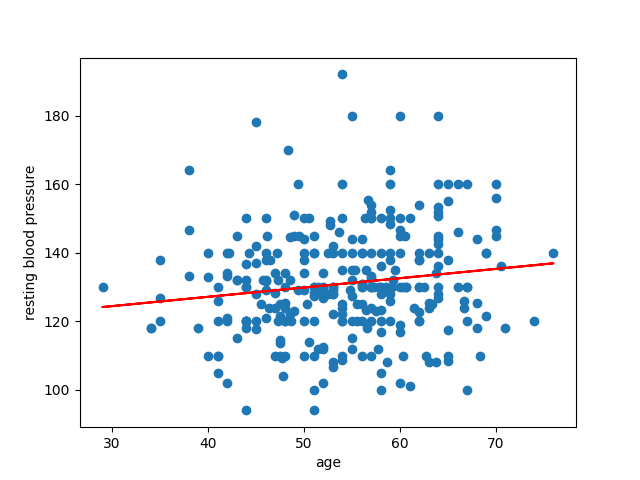
\includegraphics
                    [width=\textwidth,keepaspectratio]
                    {img/regression-30-Interpolation-resting-blood-pressure-age.png}
                    \caption
                    [regression-30-Interpolation-resting-blood-pressure-age]
                    {Współczynnik kierunkowy: 0.2714, Punkt przecięcia: 116.274}
                    \label{regression-30-Interpolation-resting-blood-pressure-age}
                \end{figure}
                \FloatBarrier

                \begin{figure}[!htbp]
                    \centering
                    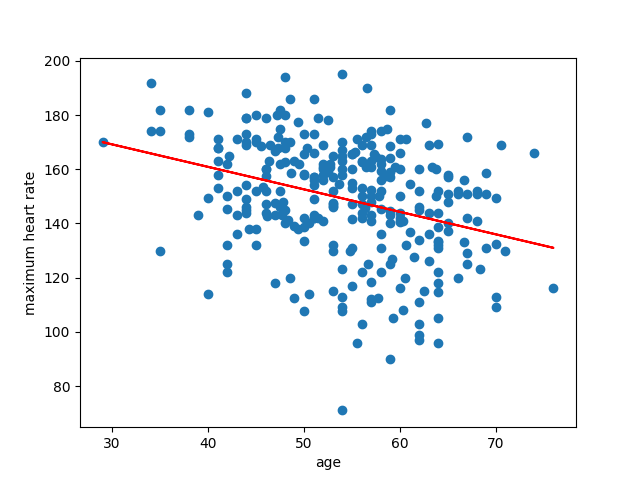
\includegraphics
                    [width=\textwidth,keepaspectratio]
                    {img/regression-30-Interpolation-maximum-heart-rate-age.png}
                    \caption
                    [regression-30-Interpolation-maximum-heart-rate-age]
                    {Współczynnik kierunkowy: -0.83, Punkt przecięcia: 194.0758}
                    \label{regression-30-Interpolation-maximum-heart-rate-age}
                \end{figure}
                \FloatBarrier

            }

            \subsubsection{Hot deck}
            \label{results:30-percent:dot-deck} {
                \begin{table}[!htbp]
                    \centering
                    \begin{tabular}{|c|c|c|c|c|c|c|}
                        \hline
                        & Mean & Std & Mode & Q1 & Median & Q3 \\ \hline
                        age & 54.7228 & 8.7464 & 55.0 & 50.0 & 55.0 & 60.0 \\ \hline
                        sex & 0.6073 & 0.4892 & 1.0 & 0.0 & 1.0 & 1.0 \\ \hline
                        chest-pain-type & 1.0363 & 1.0174 & 0.0 & 0.0 & 1.0 & 2.0 \\ \hline
                        resting-blood-pressure & 131.2574 & 16.278 & 120.0 & 120.0 & 130.0 & 140.0 \\ \hline
                        serum-cholestoral & 246.0561 & 46.8676 & 212.0 & 212.0 & 244.0 & 274.5 \\ \hline
                        fasting-blood-sugar & 0.1419 & 0.3495 & 0.0 & 0.0 & 0.0 & 0.0 \\ \hline
                        resting-electrocardiographic & 0.4785 & 0.5198 & 0.0 & 0.0 & 0.0 & 1.0 \\ \hline
                        maximum-heart-rate & 149.0759 & 22.3185 & 125.0 & 132.0 & 150.0 & 167.0 \\ \hline
                        exercise-induced-angina & 0.2739 & 0.4467 & 0.0 & 0.0 & 0.0 & 1.0 \\ \hline
                        oldpeak & 1.038 & 1.1374 & 0.0 & 0.0 & 0.8 & 1.8 \\ \hline
                        the-slope-of-the-peak-exercise & 1.3465 & 0.6372 & 1.0 & 1.0 & 1.0 & 2.0 \\ \hline
                        number-of-major-vessels & 0.7162 & 1.0351 & 0.0 & 0.0 & 0.0 & 1.0 \\ \hline
                        thal & 2.3663 & 0.5878 & 2.0 & 2.0 & 2.0 & 3.0 \\ \hline
                        target & 0.5776 & 0.4948 & 1.0 & 0.0 & 1.0 & 1.0 \\ \hline
                    \end{tabular}
                    \caption{}
                    \label{result_30_Hot-deck}
                \end{table}
                \FloatBarrier

                \begin{figure}[!htbp]
                    \centering
                    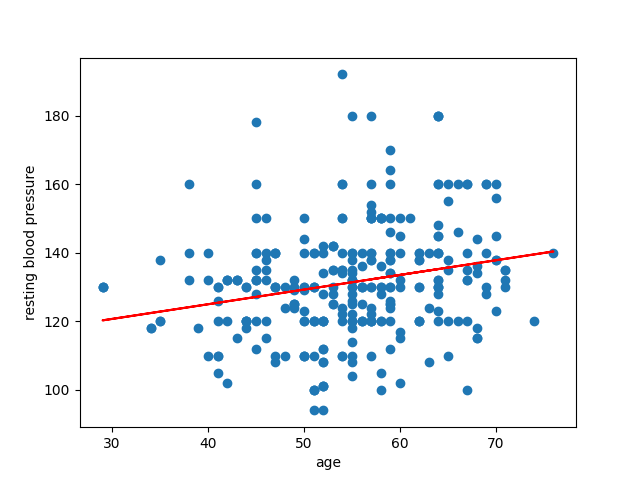
\includegraphics
                    [width=\textwidth,keepaspectratio]
                    {img/regression-30-Hot-deck-resting-blood-pressure-age.png}
                    \caption
                    [regression-30-Hot-deck-resting-blood-pressure-age]
                    {Współczynnik kierunkowy: 0.4277, Punkt przecięcia: 107.8535}
                    \label{regression-30-Hot-deck-resting-blood-pressure-age}
                \end{figure}
                \FloatBarrier

                \begin{figure}[!htbp]
                    \centering
                    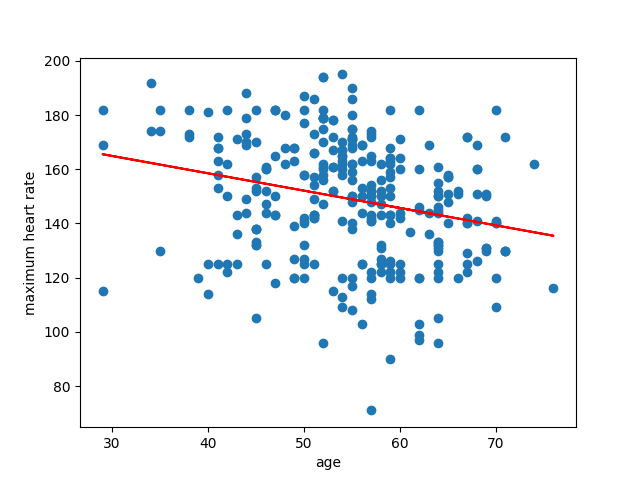
\includegraphics
                    [width=\textwidth,keepaspectratio]
                    {img/regression-30-Hot-deck-maximum-heart-rate-age.png}
                    \caption
                    [regression-30-Hot-deck-maximum-heart-rate-age]
                    {Współczynnik kierunkowy: -0.6402, Punkt przecięcia: 184.1101}
                    \label{regression-30-Hot-deck-maximum-heart-rate-age}
                \end{figure}
                \FloatBarrier

            }

            \subsubsection{Regression}
            \label{results:30-percent:regression} {

                \begin{table}[!htbp]
                    \centering
                    \begin{tabular}{|c|c|c|c|c|c|c|}
                        \hline
                        & Mean & Std & Mode & Q1 & Median & Q3 \\ \hline
                        age & 52.0441 & 8.6195 & 57.0 & 46.1239 & 51.0 & 58.0 \\ \hline
                        sex & 0.736 & 0.4415 & 1.0 & 0.0 & 1.0 & 1.0 \\ \hline
                        chest-pain-type & 0.8548 & 1.006 & 0.0 & 0.0 & 0.0 & 2.0 \\ \hline
                        resting-blood-pressure & 129.1386 & 41.7025 & 130.0 & 113.9568 & 130.0 & 140.0 \\ \hline
                        serum-cholestoral & 253.3096 & 45.0964 & 197.0 & 221.2237 & 254.0 & 283.2508 \\ \hline
                        fasting-blood-sugar & 0.1419 & 0.3495 & 0.0 & 0.0 & 0.0 & 0.0 \\ \hline
                        resting-electrocardiographic & 0.538 & 0.5189 & 1.0 & 0.0 & 1.0 & 1.0 \\ \hline
                        maximum-heart-rate & 149.7161 & 22.0882 & 152.0 & 134.8074 & 151.0 & 166.4396 \\ \hline
                        exercise-induced-angina & 0.2706 & 0.445 & 0.0 & 0.0 & 0.0 & 1.0 \\ \hline
                        oldpeak & 0.9303 & 1.007 & 0.0 & 0.0561 & 0.6791 & 1.4 \\ \hline
                        the-slope-of-the-peak-exercise & 1.462 & 0.6125 & 2.0 & 1.0 & 2.0 & 2.0 \\ \hline
                        number-of-major-vessels & 0.538 & 0.9338 & 0.0 & 0.0 & 0.0 & 1.0 \\ \hline
                        thal & 2.2508 & 0.5427 & 2.0 & 2.0 & 2.0 & 3.0 \\ \hline
                        target & 0.6535 & 0.4767 & 1.0 & 0.0 & 1.0 & 1.0 \\ \hline
                    \end{tabular}
                    \caption{}
                    \label{result_30_Regression}
                \end{table}
                \FloatBarrier

                \begin{figure}[!htbp]
                    \centering
                    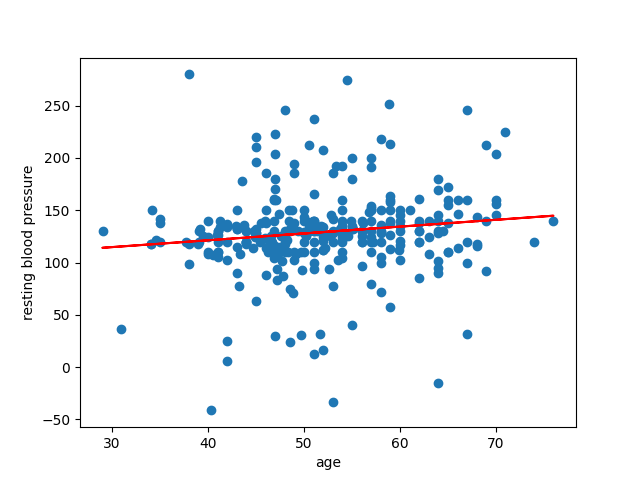
\includegraphics
                    [width=\textwidth,keepaspectratio]
                    {img/regression-30-Regression-resting-blood-pressure-age.png}
                    \caption
                    [regression-30-Regression-resting-blood-pressure-age]
                    {Współczynnik kierunkowy: 0.6523, Punkt przecięcia: 95.192}
                    \label{regression-30-Regression-resting-blood-pressure-age}
                \end{figure}
                \FloatBarrier

                \begin{figure}[!htbp]
                    \centering
                    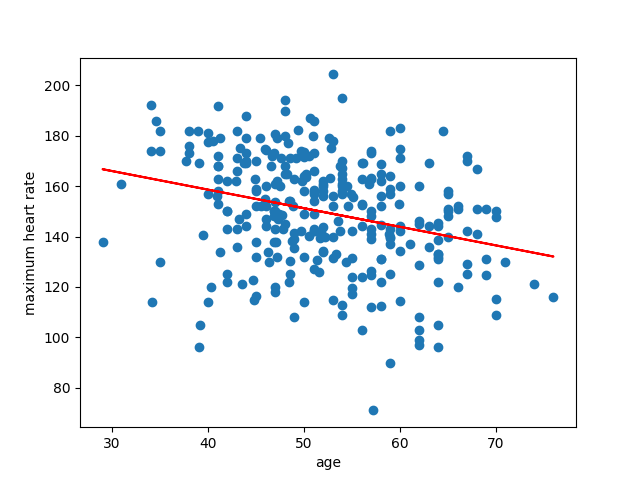
\includegraphics
                    [width=\textwidth,keepaspectratio]
                    {img/regression-30-Regression-maximum-heart-rate-age.png}
                    \caption
                    [regression-30-Regression-maximum-heart-rate-age]
                    {Współczynnik kierunkowy: -0.7374, Punkt przecięcia: 188.0914}
                    \label{regression-30-Regression-maximum-heart-rate-age}
                \end{figure}
                \FloatBarrier

            }
        }
        \newpage

        \subsection{Braki w danych 45\%}
        \label{results:45-percent} {

            \subsubsection{List wise deletion}
            \label{results:45-percent:list-wise} {
                \textit{Zbyt mało danych aby obliczyć statystyki}
            }

            \subsubsection{Mean imputation}
            \label{results:45-percent:mean-input} {
                \begin{table}[!htbp]
                    \centering
                    \begin{tabular}{|c|c|c|c|c|c|c|}
                        \hline
                        & Mean & Std & Mode & Q1 & Median & Q3 \\ \hline
                        age & 54.1198 & 6.6381 & 54.1198 & 54.0 & 54.1198 & 56.0 \\ \hline
                        sex & 0.8317 & 0.3748 & 1.0 & 1.0 & 1.0 & 1.0 \\ \hline
                        chest-pain-type & 0.9637 & 0.7427 & 1.0 & 0.0 & 1.0 & 1.0 \\ \hline
                        resting-blood-pressure & 133.2275 & 14.8216 & 133.2275 & 128.0 & 133.2275 & 137.0 \\ \hline
                        serum-cholestoral & 242.4387 & 35.148 & 242.4387 & 234.5 & 242.4387 & 242.4387 \\ \hline
                        fasting-blood-sugar & 0.099 & 0.2992 & 0.0 & 0.0 & 0.0 & 0.0 \\ \hline
                        resting-electrocar. & 0.7327 & 0.458 & 1.0 & 0.0 & 1.0 & 1.0 \\ \hline
                        maximum-heart-rate & 148.9341 & 17.4094 & 148.9341 & 148.9341 & 148.9341 & 155.0 \\ \hline
                        exercise-induced-angina & 0.2112 & 0.4089 & 0.0 & 0.0 & 0.0 & 0.0 \\ \hline
                        oldpeak & 0.9788 & 0.7814 & 0.9788 & 0.6 & 0.9788 & 0.9788 \\ \hline
                        the-slope-of-the-peak & 1.2442 & 0.5014 & 1.0 & 1.0 & 1.0 & 2.0 \\ \hline
                        number-of-major-vessels & 0.8548 & 0.8048 & 1.0 & 0.0 & 1.0 & 1.0 \\ \hline
                        thal & 2.1947 & 0.4586 & 2.0 & 2.0 & 2.0 & 2.0 \\ \hline
                        target & 0.7657 & 0.4243 & 1.0 & 1.0 & 1.0 & 1.0 \\ \hline
                    \end{tabular}
                    \caption{}
                    \label{result_45_Mean-imputation}
                \end{table}
                \FloatBarrier

                \begin{figure}[!htbp]
                    \centering
                    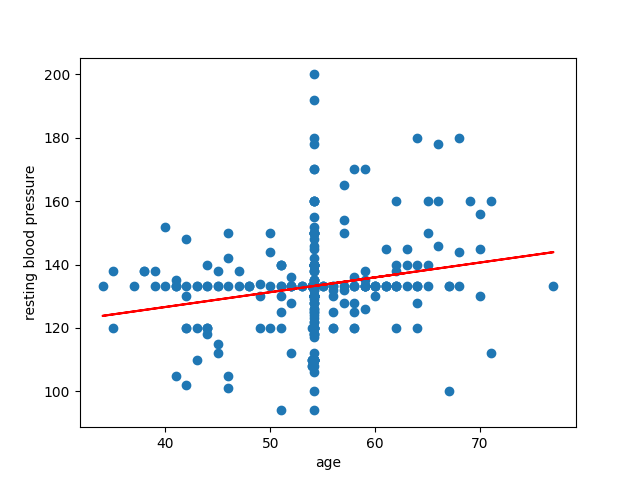
\includegraphics
                    [width=\textwidth,keepaspectratio]
                    {img/regression-45-Mean-imputation-resting-blood-pressure-age.png}
                    \caption
                    [regression-45-Mean-imputation-resting-blood-pressure-age]
                    {Współczynnik kierunkowy: 0.4675, Punkt przecięcia: 107.9272}
                    \label{regression-45-Mean-imputation-resting-blood-pressure-age}
                \end{figure}
                \FloatBarrier

                \begin{figure}[!htbp]
                    \centering
                    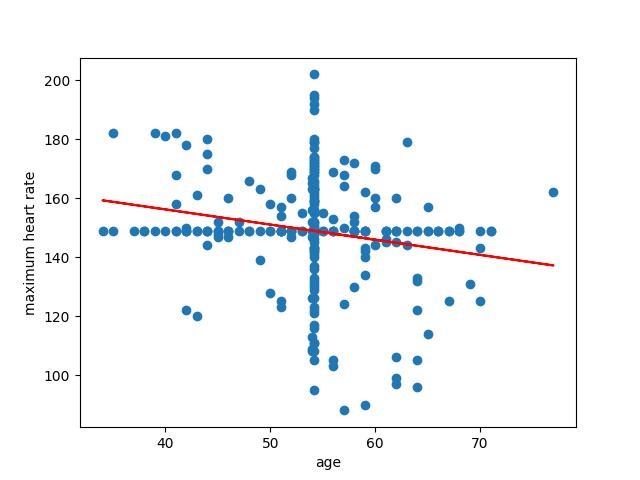
\includegraphics
                    [width=\textwidth,keepaspectratio]
                    {img/regression-45-Mean-imputation-maximum-heart-rate-age.png}
                    \caption
                    [regression-45-Mean-imputation-maximum-heart-rate-age]
                    {Współczynnik kierunkowy: -0.5138, Punkt przecięcia: 176.7426}
                    \label{regression-45-Mean-imputation-maximum-heart-rate-age}
                \end{figure}
                \FloatBarrier

            }

            \subsubsection{Interpolation}
            \label{results:45-percent:interpolation} {

                \begin{table}[!htbp]
                    \centering
                    \begin{tabular}{|c|c|c|c|c|c|c|}
                        \hline
                        & Mean & Std & Mode & Q1 & Median & Q3 \\ \hline
                        age & 54.3378 & 8.0693 & 54.0 & 49.0 & 55.0 & 60.0 \\ \hline
                        sex & 0.6622 & 0.4738 & 1.0 & 0.0 & 1.0 & 1.0 \\ \hline
                        chest-pain-type & 0.8328 & 0.9334 & 0.0 & 0.0 & 1.0 & 2.0 \\ \hline
                        resting-blood-pressure & 132.5953 & 16.9114 & 130.0 & 120.0 & 130.0 & 140.0 \\ \hline
                        serum-cholestoral & 244.2261 & 46.4819 & 226.0 & 214.5 & 238.6667 & 270.875 \\ \hline
                        fasting-blood-sugar & 0.1605 & 0.3677 & 0.0 & 0.0 & 0.0 & 0.0 \\ \hline
                        resting-electrocardiographic & 0.4247 & 0.5085 & 0.0 & 0.0 & 0.0 & 1.0 \\ \hline
                        maximum-heart-rate & 150.1438 & 21.1781 & 152.0 & 136.0 & 152.0 & 164.75 \\ \hline
                        exercise-induced-angina & 0.3211 & 0.4677 & 0.0 & 0.0 & 0.0 & 1.0 \\ \hline
                        oldpeak & 1.0065 & 0.9889 & 0.0 & 0.09 & 0.8 & 1.6 \\ \hline
                        the-slope-of-the-peak-exercise & 1.4381 & 0.6009 & 2.0 & 1.0 & 1.0 & 2.0 \\ \hline
                        number-of-major-vessels & 0.6756 & 0.9685 & 0.0 & 0.0 & 0.0 & 1.0 \\ \hline
                        thal & 2.3344 & 0.5512 & 2.0 & 2.0 & 2.0 & 3.0 \\ \hline
                        target & 0.5385 & 0.4994 & 1.0 & 0.0 & 1.0 & 1.0 \\ \hline
                    \end{tabular}
                    \caption{}
                    \label{result_45_Interpolation}
                \end{table}
                \FloatBarrier

                \begin{figure}[!htbp]
                    \centering
                    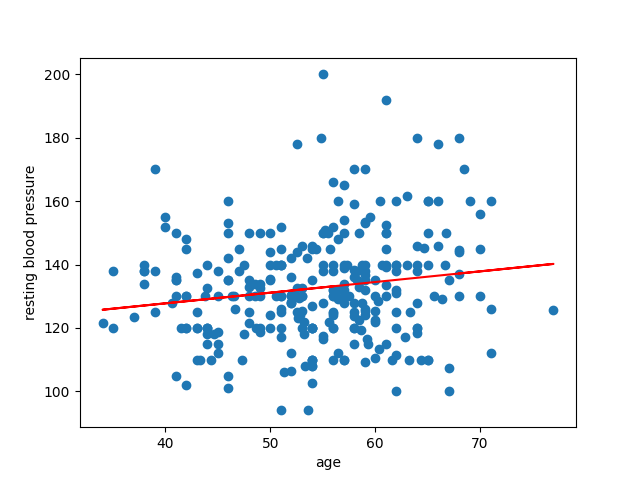
\includegraphics
                    [width=\textwidth,keepaspectratio]
                    {img/regression-45-Interpolation-resting-blood-pressure-age.png}
                    \caption
                    [regression-45-Interpolation-resting-blood-pressure-age]
                    {Współczynnik kierunkowy: 0.3362, Punkt przecięcia: 114.328}
                    \label{regression-45-Interpolation-resting-blood-pressure-age}
                \end{figure}
                \FloatBarrier

                \begin{figure}[!htbp]
                    \centering
                    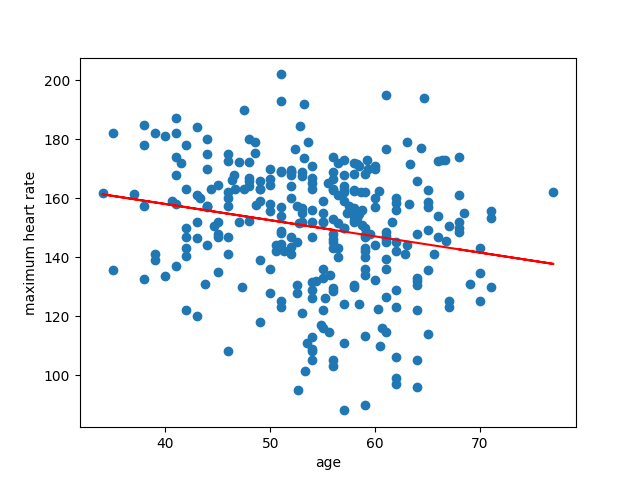
\includegraphics
                    [width=\textwidth,keepaspectratio]
                    {img/regression-45-Interpolation-maximum-heart-rate-age.png}
                    \caption
                    [regression-45-Interpolation-maximum-heart-rate-age]
                    {Współczynnik kierunkowy: -0.5493, Punkt przecięcia: 179.9911}
                    \label{regression-45-Interpolation-maximum-heart-rate-age}
                \end{figure}
                \FloatBarrier

            }

            \subsubsection{Hot deck}
            \label{results:45-percent:dot-deck} {
                \begin{table}[!htbp]
                    \centering
                    \begin{tabular}{|c|c|c|c|c|c|c|}
                        \hline
                        & Mean & Std & Mode & Q1 & Median & Q3 \\ \hline
                        age & 52.5281 & 8.9468 & 44.0 & 44.0 & 53.0 & 59.0 \\ \hline
                        sex & 0.6568 & 0.4756 & 1.0 & 0.0 & 1.0 & 1.0 \\ \hline
                        chest-pain-type & 1.0462 & 0.972 & 0.0 & 0.0 & 1.0 & 2.0 \\ \hline
                        resting-blood-pressure & 132.6073 & 17.6662 & 120.0 & 120.0 & 130.0 & 140.0 \\ \hline
                        serum-cholestoral & 240.6436 & 43.6327 & 216.0 & 216.0 & 234.0 & 265.0 \\ \hline
                        fasting-blood-sugar & 0.1749 & 0.3805 & 0.0 & 0.0 & 0.0 & 0.0 \\ \hline
                        resting-electrocardiographic & 0.4983 & 0.5139 & 0.0 & 0.0 & 0.0 & 1.0 \\ \hline
                        maximum-heart-rate & 153.7822 & 21.2241 & 171.0 & 143.0 & 159.0 & 170.0 \\ \hline
                        exercise-induced-angina & 0.3993 & 0.4906 & 0.0 & 0.0 & 0.0 & 1.0 \\ \hline
                        oldpeak & 0.9323 & 0.9955 & 0.0 & 0.0 & 0.8 & 1.5 \\ \hline
                        the-slope-of-the-peak-exercise & 1.5347 & 0.5794 & 2.0 & 1.0 & 2.0 & 2.0 \\ \hline
                        number-of-major-vessels & 0.5248 & 0.9377 & 0.0 & 0.0 & 0.0 & 1.0 \\ \hline
                        thal & 2.3135 & 0.5374 & 2.0 & 2.0 & 2.0 & 3.0 \\ \hline
                        target & 0.6634 & 0.4733 & 1.0 & 0.0 & 1.0 & 1.0 \\ \hline
                    \end{tabular}
                    \caption{}
                    \label{result_45_Hot-deck}
                \end{table}
                \FloatBarrier

                \begin{figure}[!htbp]
                    \centering
                    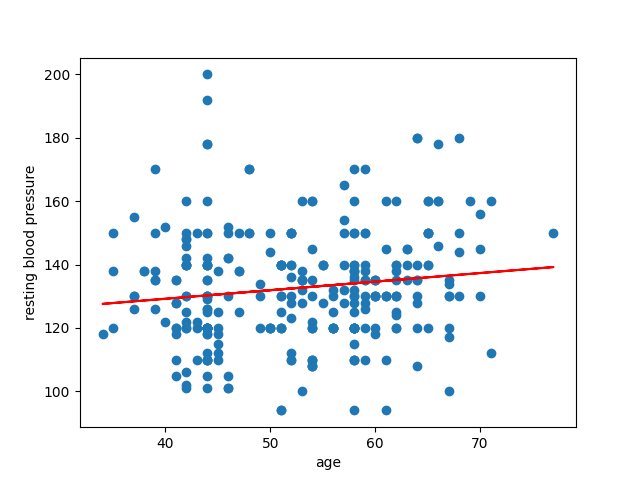
\includegraphics
                    [width=\textwidth,keepaspectratio]
                    {img/regression-45-Hot-deck-resting-blood-pressure-age.png}
                    \caption
                    [regression-45-Hot-deck-resting-blood-pressure-age]
                    {Współczynnik kierunkowy: 0.2702, Punkt przecięcia: 118.4117}
                    \label{regression-45-Hot-deck-resting-blood-pressure-age}
                \end{figure}
                \FloatBarrier

                \begin{figure}[!htbp]
                    \centering
                    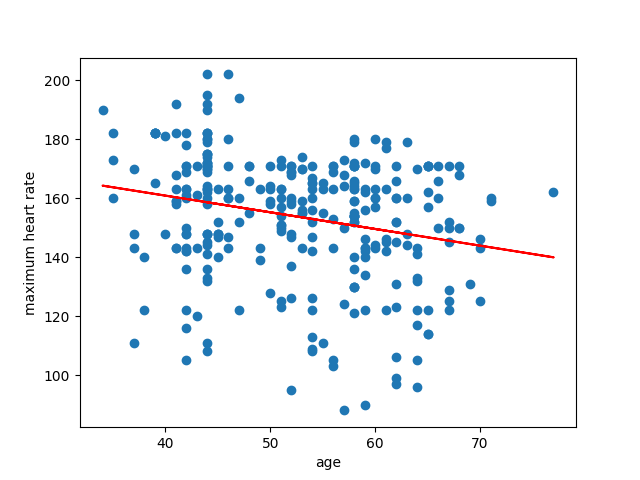
\includegraphics
                    [width=\textwidth,keepaspectratio]
                    {img/regression-45-Hot-deck-maximum-heart-rate-age.png}
                    \caption
                    [regression-45-Hot-deck-maximum-heart-rate-age]
                    {Współczynnik kierunkowy: -0.5656, Punkt przecięcia: 183.4912}
                    \label{regression-45-Hot-deck-maximum-heart-rate-age}
                \end{figure}
                \FloatBarrier

            }

            \subsubsection{Regression}
            \label{results:45-percent:regression} {
                \textit{Zbyt mało danych aby utworzyć model regresji liniowej}
            }
        }
    }

    \section{Dyskusja}
    \label{summary} {

        \subsubsection{Mean imputation}
        \label{summary:mean-input} {
            Metoda \textit{Mean inputation} polega na uzupełnianiu brakujących wartości średnią 
            danej kolumny.
        
            Porównując wyniki uzyskane z użyciem metody \textit{Mean inputation} a
            \textit{List wise deletion} dla braków na poziomie 5\% można zauważyć delikatny
            wzrost wartości a co za tym idzie wartości \textit{Q1}, \textit{Mediany} oraz \textit{Q3} uległy też zmianie.
            Bardzo ciekawą obserwacją jest to, że wartość mody(dominanty) \textit{serum-cholestoral} jest
            teraz równa średniej arytmetycznej. Krzywe regresji są do siebie mocno zbliżone,
            ze względu na fakt, że zbiory są bardzo podobne do siebie.
            
            W przypadku braków na poziomie 15\% zauważa się coraz większy wzrost wartości 
            w porównaniu do braków na poziomie 5\%. Jedyną kolumną odbiegającą od tej 
            tendencji jest \textit{maximum-heart-rate} gdzie wartość wszystkich miar 
            statystycznych zmalała. Krzywe regresji diametralnie się od siebie różnią, 
            jest to spowodowane tym, że w \textit{List wise deletion} jest znacząco 
            mniej rekordów, dla tych kolumn, które są wizualizowane na
            wykresach - liczba punktów na wykresie.
            
            W przypadku braków na poziomie 30\% sytuacja coraz bardziej się pogłębia 
            i wygenerowane dane w bardzo słaby sposób wypełniają istniejące braki. W tym 
            przypadku porównywanie krzywych regresji w ocenie autora nie jest sensowne ze
            względu na liczbę punktów na wykresach dla metody \textit{List wise deletion}.
            
            Dla przypadków braków na poziomie 15\% i 30\% można zauważyć, że dla wielu 
            kolumn wartości średniej i mody są takie same. Można wnioskować, że
            większość wartości w danej kolumnie jest identyczna.
            
            W przypadku braków na poziomie 45\% nie ma możliwości porównania do 
            gdyż \textit{List wise deletion} danych było tak mało, że nie było możliwości 
            wyliczenia statystyk.
        }

        \subsubsection{Interpolation}
        \label{summary:interpolation} {
            Metoda interpolacji polega na uzupełnieniu brakujących danych średnią,
            wyliczaną z dwóch niepustych rekordów, które sąsiadują z usuniętą wartością.

            Pomimo faktu dużej ilości braku, interpolacja bazuje na wartościach
            obliczanych lokalnie, stąd brak istotnych odchyleń w otrzymanych wynikach.
            Wraz ze zwiększaniem procent imputowanych danych, maleje odchylenie
            standardowe, co jest efektem obliczania brakujących wartości za pomocą
            interpolacji liniowej. Analizując krzywe regresji można zauważyć, iż jest
            to metoda, która poradziła sobie poprawnie w uzupełnianiu danych.

            Porównując skrajne przykłady zbiorów wybrakowanych w 5\% i w 45\% można
            zauważyć, że nawet w przypadku dużego stopnia wybrakowania metoda
            interpolacji osiąga zbliżone wyniki.
        }

        \subsubsection{Hot deck}
        \label{summary:dot-deck} {
            Metoda hot deck polega na uzupełnieniu brakujących danych wartościami,
            pochodzącymi z najbardziej podobnego rekordu. Oczywiście pojęcie "podobny"
            jest zupełnie względne, w tym przypadku odnosi się ono do odległości euklidesowej.

            W przypadku zbioru danych wybrakowanym na poziomie 5\% trudno dostrzec
            jakieś specjalne różnice między statystykami wyliczonymi po imputacji
            metodą hot deck, a przed jakąkolwiek imputacją. Kwartyle pozostały
            zbliżone, średnia i odchylenie standardowe również nie uległy zauważalnym
            zmianom. Chyba najbardziej widoczna różnica dotyczy wartości mody. Ta
            bowiem nie powinna zmieniać się zbyt łatwo, jako że oznacza najczęściej
            występującą wartość. Okazuje się jednak, że prawie w każdej kolumnie uległa
            zmianie, w niektórych w dość radykalny sposób (jak np. dla
            serum-cholestoral). Zjawisko to można w miarę łatwo wyjaśnić, kiedy spojrzy
            się na różnicę w wykresach krzywej regresji. Zdecydowanie widać tutaj, że w
            zbiorze po imputacji, spora część wartości się powtarza. Tak więc rekordy
            uznane za najbardziej podobne stanowią jakąś niewielką grupę i są często
            wykorzystywane jako "dawcy" brakującej wartości. Jako że brakująca wartość
            często jest brana z tego samego rekordu zaczyna ona często występować i w
            rezultacie zaczyna pełnić rolę mody. Fakt, że niektóre rekordy najczęściej
            są dawcami, może być spowodowany tym, że dane nie zostały znormalizowane i
            atrybuty o dużych wartościach mają zdecydowanie większy wpływ na podobieństwo.

            Zjawisko to potwierdza się i nasila w przypadku bardziej wybrakowanych
            zbiorów. Dodatkowo zaczyna zwiększać się różnica także w innych
            statystykach. W zbiorze wybrakowanym na poziomie 15\% zaczyna być widoczny
            sens imputowania danych. Statystyki dla zbioru przed imputacją różnią się
            znacznie od tych przed imputacją dla zbioru wybrakowanego w 5\%. Jednakże
            Po imputacji metodą hot deck, statystyki znowu są zbliżone do tych w
            zbiorze mało wybrakowanym. Krzywe regresji od poziomu wybrakowania 15\%
            stały się zupełnie bez wartości, dla danych bez imputacji. Na tym poziomie
            po imputacji współczynniki są wciąż zbliżone do oryginalnych. Choć różnica
            staje się coraz większa dla poziomu 30\%, krzywe po imputacji wciąż
            zachowują ten sam kierunek a statystyki ten sam rząd. W przypadku
            wybrakowania na najwyższym poziomie, na wykresach wyraźnie widać, że mamy
            tutaj tylko kilku "dawców" i wartości, które przyjmują poszczególne
            atrybuty są zdecydowanie skwantyzowane. Nie przeszkadza to jednak w
            zachowaniu wciąż podobnych do zbioru niewybrakowanego wartości statystyk.
            Ostatecznie należy więc powiedzieć, że metoda hot-deck jest dość skuteczna
            nawet przy dużym poziomie wybrakowania zbioru, w przeciwieństwie bowiem do
            metody mean-imputation, nie jest podatna na silne zmiany rozkładu wartości
            atrybutów, w wybrakowanym zbiorze.

        }

        \subsubsection{Regression}
        \label{summary:regression} {
            Metoda wykorzystująca krzywą regresji, polega na stworzeniu modelu
            regresji, wykorzystując do tego dostępne dane bez braków. Na podstawie tego
            modelu ustalone zostają wartości brakujących atrybutów. W zależności od
            rodzaju danych zostały wykorzystane różne rodzaje regresji. Do ustalenia
            wartości atrybutów, których wartość należała do zbioru określonych
            wartości, jak np. płeć, wykorzystywana była regresja logistyczna, w
            realizacji pozostałych przypadków wystarczała regresja liniowa. Do
            poprawnego działania metoda wymaga znacznej liczby parametrów, przez co
            niemożliwe okazało się wykorzystanie tej metody dla zbiorów, których liczba
            brakujących danych wynosiła 45\%

            Wykorzystując zgromadzone statystyki można stwierdzić, że zastosowanie
            krzywej regresji, jako metody imputacji, w największym stopniu wpłynie na
            zmianę wartości mody (dominanty), im większy procent braku danych tym
            różnica jest bardziej widoczna. Warto jednak zauważyć, że wartość mediany,
            nie jest tak podatna na zmiany, przy wykorzystaniu tej metody.
        }

    }

    \section{Wnioski}
    \label{conclusions} {
        Podsumowując wykonane zadanie wnioskujemy, że:
        \begin{itemize}
            \item Metody \textit{Mean inputation} sprawdza się dobrze dla małych ubytków
            w danych w dużych zbiorach, które nie posiadają dużej liczby wartości
            ekstremalnych. Ze względu na charakterystykę średniej wartości mogą bardzo
            zaburzyć imputacje.
            \item Przy dużym procencie brakujących danych, należy rozważyć odrzucenie
            próby analizy danych, zawartych w tym zbiorze, z powodu trudności,
            jaką jest uzupełnienie danych. Przy dużym braku danych, każda z metod
            imputacji w sposób znaczący wpłynie na statystyki zbioru, przy
            założeniu, że uda się ją zastosować.
            \item Metoda hot deck sprawdza się stosunkowo dobrze przy dużym poziomie
            wybrakowania zbioru, implementacyjnie jest jednak znacznie bardzie
            skomplikowana niż np mean-imputation

        \end{itemize}
    }

    \begin{thebibliography}{0}
        \bibitem{dataset}{https://www.kaggle.com/ronitf/heart-disease-uci}
    \end{thebibliography}

\end{document}
